\chapter{脑机接口} \label{chap:chap39}

了解神经系统的正常功能对于了解疾病或损伤引起的功能障碍以及设计疗法至关重要。
此类治疗包括药物制剂、外科手术以及越来越多的电子医疗设备。
这些医疗设备填补了主要分子靶向和全身药物治疗与主要解剖学靶向和局灶性手术损伤之间的重要空白。


在本章中,我们重点关注在神经元群体水平上测量或改变电生理活动的医疗设备。
这些设备被称为脑机接口 (BMI)、脑机接口或神经假体。
我们使用术语脑机接口来指代所有此类设备,因为它们之间没有标准区别。
脑机接口可分为四大类:恢复失去的感觉能力的脑机接口、恢复失去的运动能力的脑机接口、调节病理性神经活动的脑机接口以及恢复失去的大脑处理能力的脑机接口。


脑机接口可以帮助人们进行“日常生活活动”,例如自己吃饭、穿衣打扮、保持自制和行走。
我们将在本章中广泛讨论的一种脑机接口将大脑神经元的电活动转换为控制假肢装置以帮助瘫痪患者的信号。
通过了解神经科学和神经工程学如何共同创造当前的脑机接口,我们可以更清楚地设想有多少神经系统疾病和损伤可以用医疗设备治疗。



\section{脑机接口测量和调节神经活动以帮助恢复失去的能力}

\subsection{运动和通信脑机接口可以恢复失去的运动能力}

最早和最广泛使用的脑机接口之一是人工耳蜗。
重度耳聋的人甚至可以从恢复部分听力中获益。
自二十世纪七十年代以来,数十万因外周性耳聋导致耳蜗神经和中枢听觉通路完好无损的人接受了人工耳蜗植入。 
这些系统已经恢复了相当大的听力和口语能力,甚至对于已经学会使用人工耳蜗来感知语言的先天性耳聋儿童也是如此。


人工耳蜗的工作原理是使用位于皮肤外部的麦克风捕捉声音,并将这些信号发送到通过手术植入耳朵附近皮肤下的接收器。
在转换(编码)为适当的时空信号模式后,这些信号电刺激耳蜗蜗轴中的螺旋神经节细胞(第 ~\ref{chap:chap26}~章)。
反过来,来自激活的耳蜗细胞的信号通过听觉神经传输到脑干和更高的听觉区域,理想情况下,神经信号被解释为麦克风捕获的声音。


脑机接口的另一个例子是视网膜假体。
失明可能由色素性视网膜炎(一种遗传性视网膜退行性疾病)等疾病引起。
目前,没有治愈方法,也没有批准的药物疗法可以减缓或逆转这种疾病。
视网膜假体目前使患者能够识别大字母并定位物体的位置。
它们通过使用相机捕捉图像并将这些信号发送到位于眼睛内的接收器来操作。
在转换为适当的时空模式后,这些电信号通过数十个电极刺激视网膜中的视网膜神经节细胞。
反过来,这些细胞通过视神经将它们的信号发送到丘脑和更高的视觉区域,理想情况下,传入信号被解释为相机捕获的图像。



\subsection{运动和通信脑机接口可以恢复失去的运动能力}

还正在开发脑机接口,以通过恢复失去的运动和通信功能来帮助瘫痪者和截肢者。
这是本章的中心话题。
首先,使用放置在初级运动皮层、背侧和腹侧前运动皮层和/或顶内皮层(特别是顶叶范围)的手臂和手部区域的穿透性多电极阵列测量一个或多个大脑区域的电神经活动 区和内侧顶内区)(图~\ref{fig:39_1})。


\begin{figure}[htbp]
	\centering
	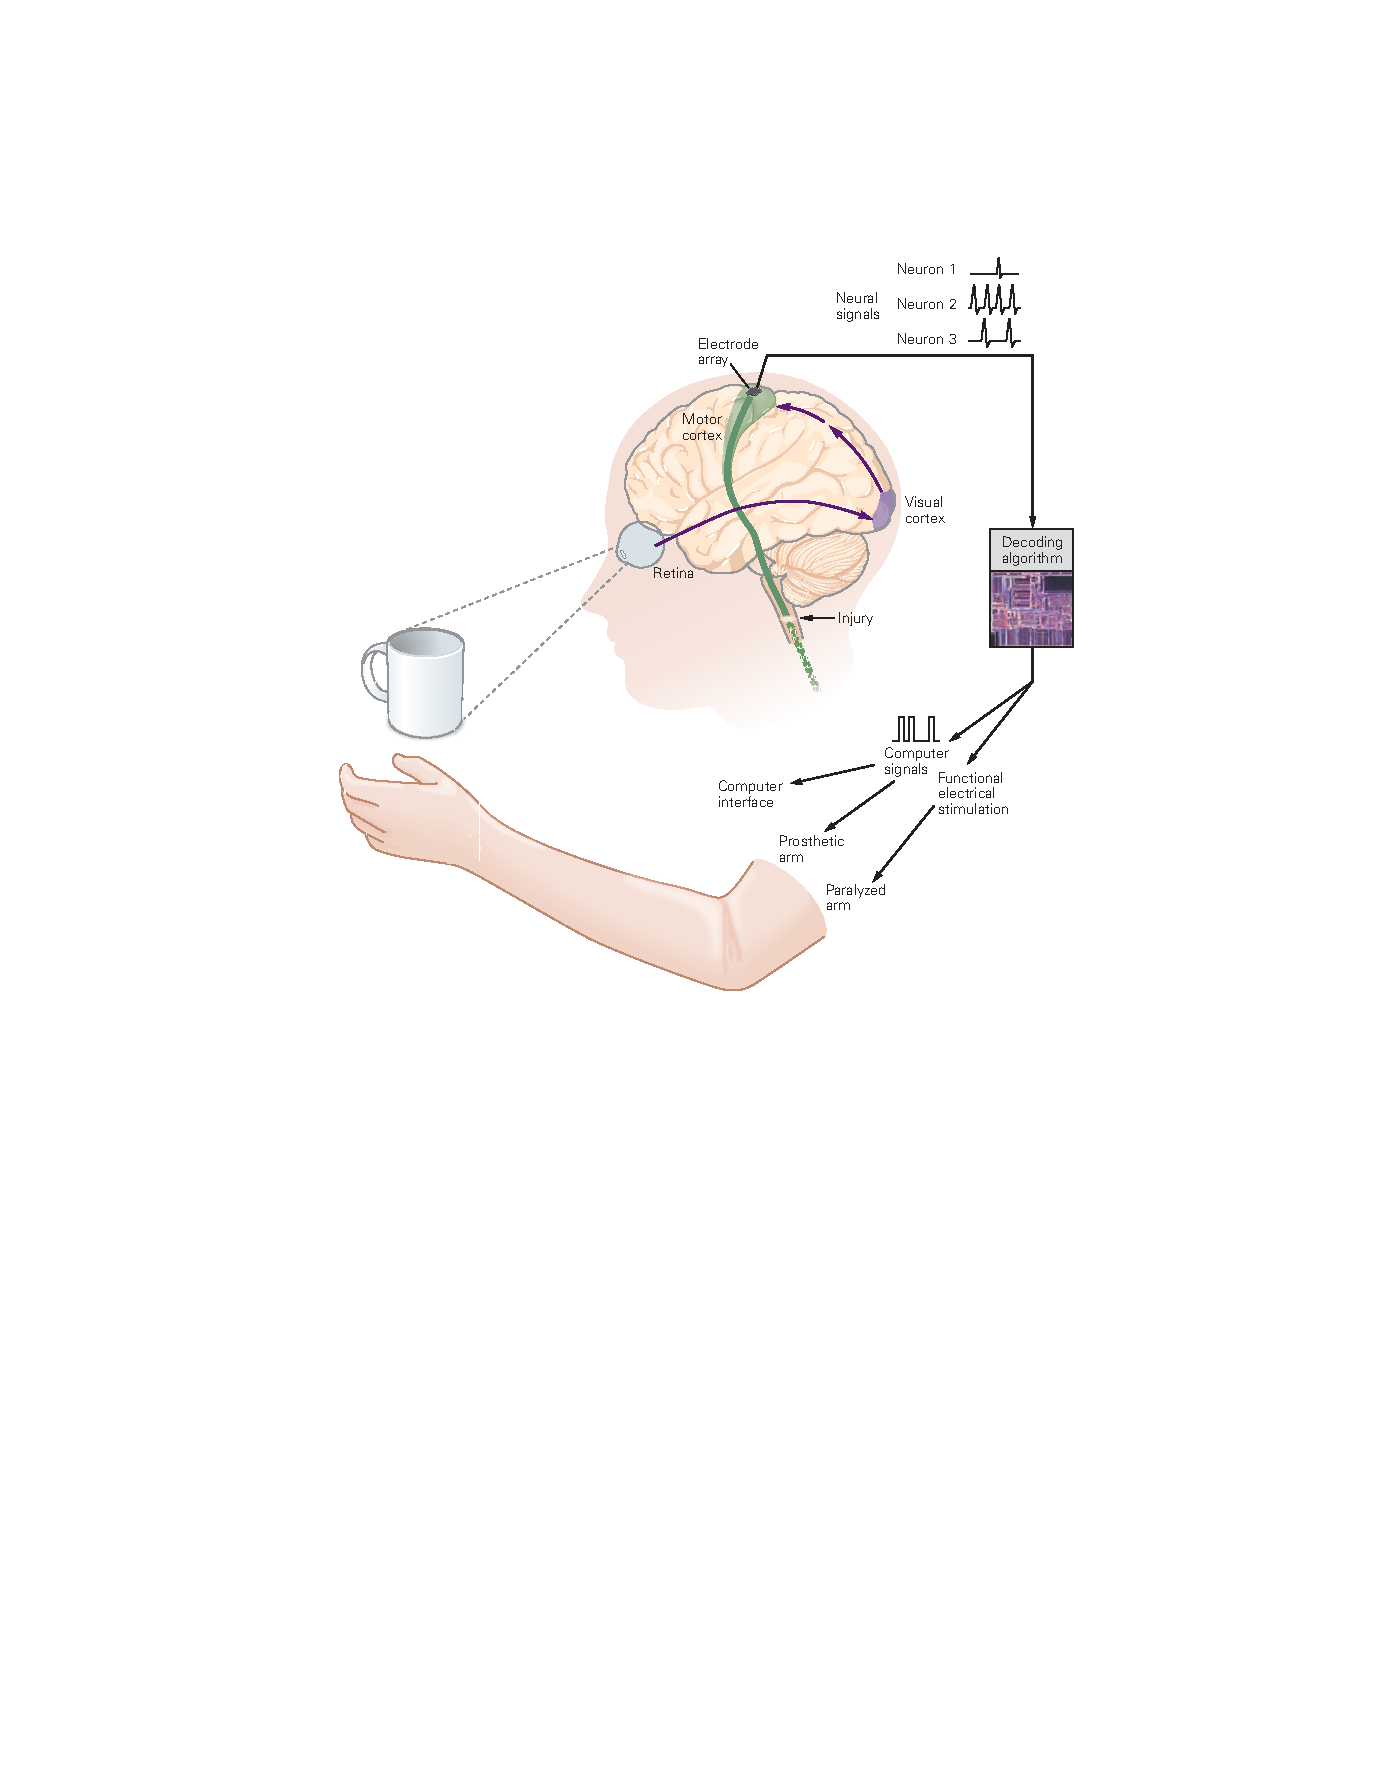
\includegraphics[width=0.5\linewidth]{chap39/fig_39_1}
	\caption{运动和通信脑机接口的概念。
		一个或多个电极阵列被植入大脑区域,例如初级运动皮层、背侧和腹侧运动前皮层或顶内皮层。
		他们记录了数十到数百个神经元的动作电位和局部场电位。
		然后,通过解码算法将记录的神经活动转换为 (1) 用于控制计算机界面或假肢(机器人)手臂的计算机命令,或 (2) 用于对瘫痪手臂肌肉进行功能性电刺激的刺激模式。}
	\label{fig:39_1}
\end{figure}


其次,尝试手臂运动,但对于瘫痪的人来说是不可能的。 
在这些尝试中测量动作电位和局部场电位。
例如,将 100 个电极放置在初级运动皮层中,另外 100 个电极放置在背侧前运动皮层中,测量来自大约 200 个神经元的动作电位和来自 200 个电极的局部场电位。
局部场电位是记录在与动作电位相同的电极上的低频信号,并且被认为是由电极尖端附近的许多神经元的局部突触电流引起的。
这些神经信号一起包含了有关该人希望如何移动她的手臂的大量信息。


第三,表征了神经活动与尝试运动之间的关系。
这种关系使得从新的神经活动预测所需的运动成为可能,我们称之为神经解码的统计过程。
第四,然后脑机接口在其正常模式下运行,实时测量神经活动,并通过计算机从神经活动中解码所需的运动。
解码后的运动可用于引导假肢设备,例如计算机屏幕上的光标或机械臂。
还可以对瘫痪肢体的肌肉进行电刺激以进行解码运动,这一过程称为功能性电刺激。
随着我们越来越多地与我们周围的世界进行电子交互(例如,智能手机、汽车和嵌入电子设备以便它们可以发送和接收数据的日常用品——称为“物联网”),可以设想许多其他假肢设备 )。


最后,因为人可以看到假肢装置,她可以通过每时每刻思考不同的想法来改变自己的神经活动,从而更准确地引导假肢装置。
这种闭环反馈控制系统也可以利用非视觉感觉方式,包括从包裹在或嵌入假肢中的电子传感器传递压力和位置信息。
这种替代感觉信息可以转化为电刺激模式,传递到本体感受和体感皮层。


上述脑机接口包括运动和通讯脑机接口。
电机脑机接口旨在提供对机器人肢体或瘫痪肢体的自然控制。
在上肢假肢的情况下,这涉及到手臂沿着所需路径并以所需速度进行精确运动。
这种控制确实是一个雄心勃勃的最终目标,但即使是实现这一目标的中间步骤也可以通过恢复一些失去的运动功能和提高患者进行“日常生活活动”的能力来改善生活质量。
例如,许多四肢瘫痪的人可以从能够自己养活中受益。


通信脑机接口旨在为大量电子设备提供快速准确的接口。 
在屏幕键盘上移动计算机光标的能力允许患者为计算机、智能手机、语音合成器、智能家居和“物联网”键入命令。 
理想情况下,通信脑机接口将允许大多数人说话或打字的通信速率。
这样的脑机接口将使患有肌萎缩侧索硬化症 (ALS) 的人受益,他们经常被“锁在里面”并且无法通过任何运动与外界交流。
交流脑机接口也将使患有严重损害运动和言语质量的其他神经退行性疾病的人以及上脊髓损伤的人受益。
每分钟可靠地键入多个单词的能力对于许多患者的生活质量来说是一种有意义的改善。


运动和交流脑机接口建立在自主运动的基础神经科学研究之上(第~\ref{chap:chap34}~章)。 
迄今为止,脑机接口的设计和开发依赖于实验室动物研究,主要是非人类灵长类动物;
然而,最近,针对瘫痪患者的临床试点试验已经开始。



\subsection{病理性神经活动可以通过深部脑刺激和抗癫痫脑机接口来调节}

脑机接口已被开发用于帮助患有涉及大脑病理性神经活动的疾病的人,例如帕金森病和癫痫症。
帕金森病患者因减少手和手臂震颤而受益。 
目前,帕金森病尚无治愈方法,许多人对药物治疗产生抗药性。
深部脑刺激器 (DBS) 可以通过向大脑中的目标区域输送电脉冲来破坏异常的神经活动,从而帮助这些人。


DBS 由植入胸部的神经刺激器控制,该神经刺激器通过电线连接到深部脑核(例如丘脑底核)中的刺激电极。 
这些电极不断地刺激细胞核,以改变异常的神经活动。 
这种方法通常可以大大减少帕金森病相关的震颤多年。 
应用于不同大脑区域的 DBS 还可以帮助患有特发性震颤、肌张力障碍、慢性疼痛、重度抑郁症和强迫症的人。


数以百万计的癫痫发作患者目前正在接受抗癫痫药物治疗或神经外科手术,这两种方法通常都无法完全或暂时减少癫痫发作。
抗癫痫脑机接口已显示出进一步改善生活质量的巨大希望。 
这些完全植入的脑机接口通过持续监测确定与癫痫发作有关的大脑区域的神经活动来运作。 
他们识别出可预测癫痫发作的异常活动,然后在几毫秒内做出反应,通过电刺激相同或不同的大脑区域来破坏这种活动。 
这种闭环反应可以足够快,以至于感觉不到癫痫发作症状并且不会发生癫痫发作。



\subsection{替换零件脑机接口可以恢复失去的大脑处理能力}

脑机接口能够恢复的不仅仅是失去的感觉或运动能力。
原则上,它们能够恢复内部大脑处理。
在四类脑机接口中,这是最具未来感的。
一个例子是“替换零件”脑机接口。
中心思想是,如果对大脑区域的功能有足够的了解,并且如果该区域因疾病或受伤而受损,那么就有可能替换该大脑区域。


一旦测量到大脑区域的正常输入活动(见下一节),就可以在电子硬件和软件中对丢失的大脑区域的功能进行建模,然后来自该替代处理中心的输出将被传送到下一个大脑区域,就像没有发生伤害一样。
这将涉及,例如,用电极读取神经活动,用低功率微电子回路模拟大脑区域的计算功能,然后用刺激电极写入电神经活动。


此过程也可用于启动和指导神经可塑性。
目前正在研究的替换部分脑机接口侧重于通过替换因受伤或疾病而受损的海马体部分来恢复记忆。
另一个潜在的应用是恢复因中风受损的大脑区域失去的功能。


这些系统代表了脑机接口概念的自然演变,即所谓的“平台技术”,因为可以通过混合和匹配各种写入、计算和读出组件来设想大量系统。
随着我们对神经系统功能的了解和技术的不断成熟,脑机接口应该能够帮助解决的神经系统疾病和损伤的数量应该会增加。



\subsection{测量和调节神经活动依赖于先进的神经技术}

测量和调节神经活动涉及应用于神经系统的电子技术的四个广泛领域(所谓的神经技术)。
第一个区域是神经传感器的类型;
人工神经传感器的设计具有不同程度的侵入性和空间分辨率(图~\ref{fig:39_2})。
近几十年来,身体外部的传感器已被广泛使用,例如脑电图 (EEG) 帽。 脑电图测量来自许多应用于头部头皮表面的小金属盘(电极)的信号。
每个电极检测其下方大量神经元的平均活动。


\begin{figure}[htbp]
	\centering
	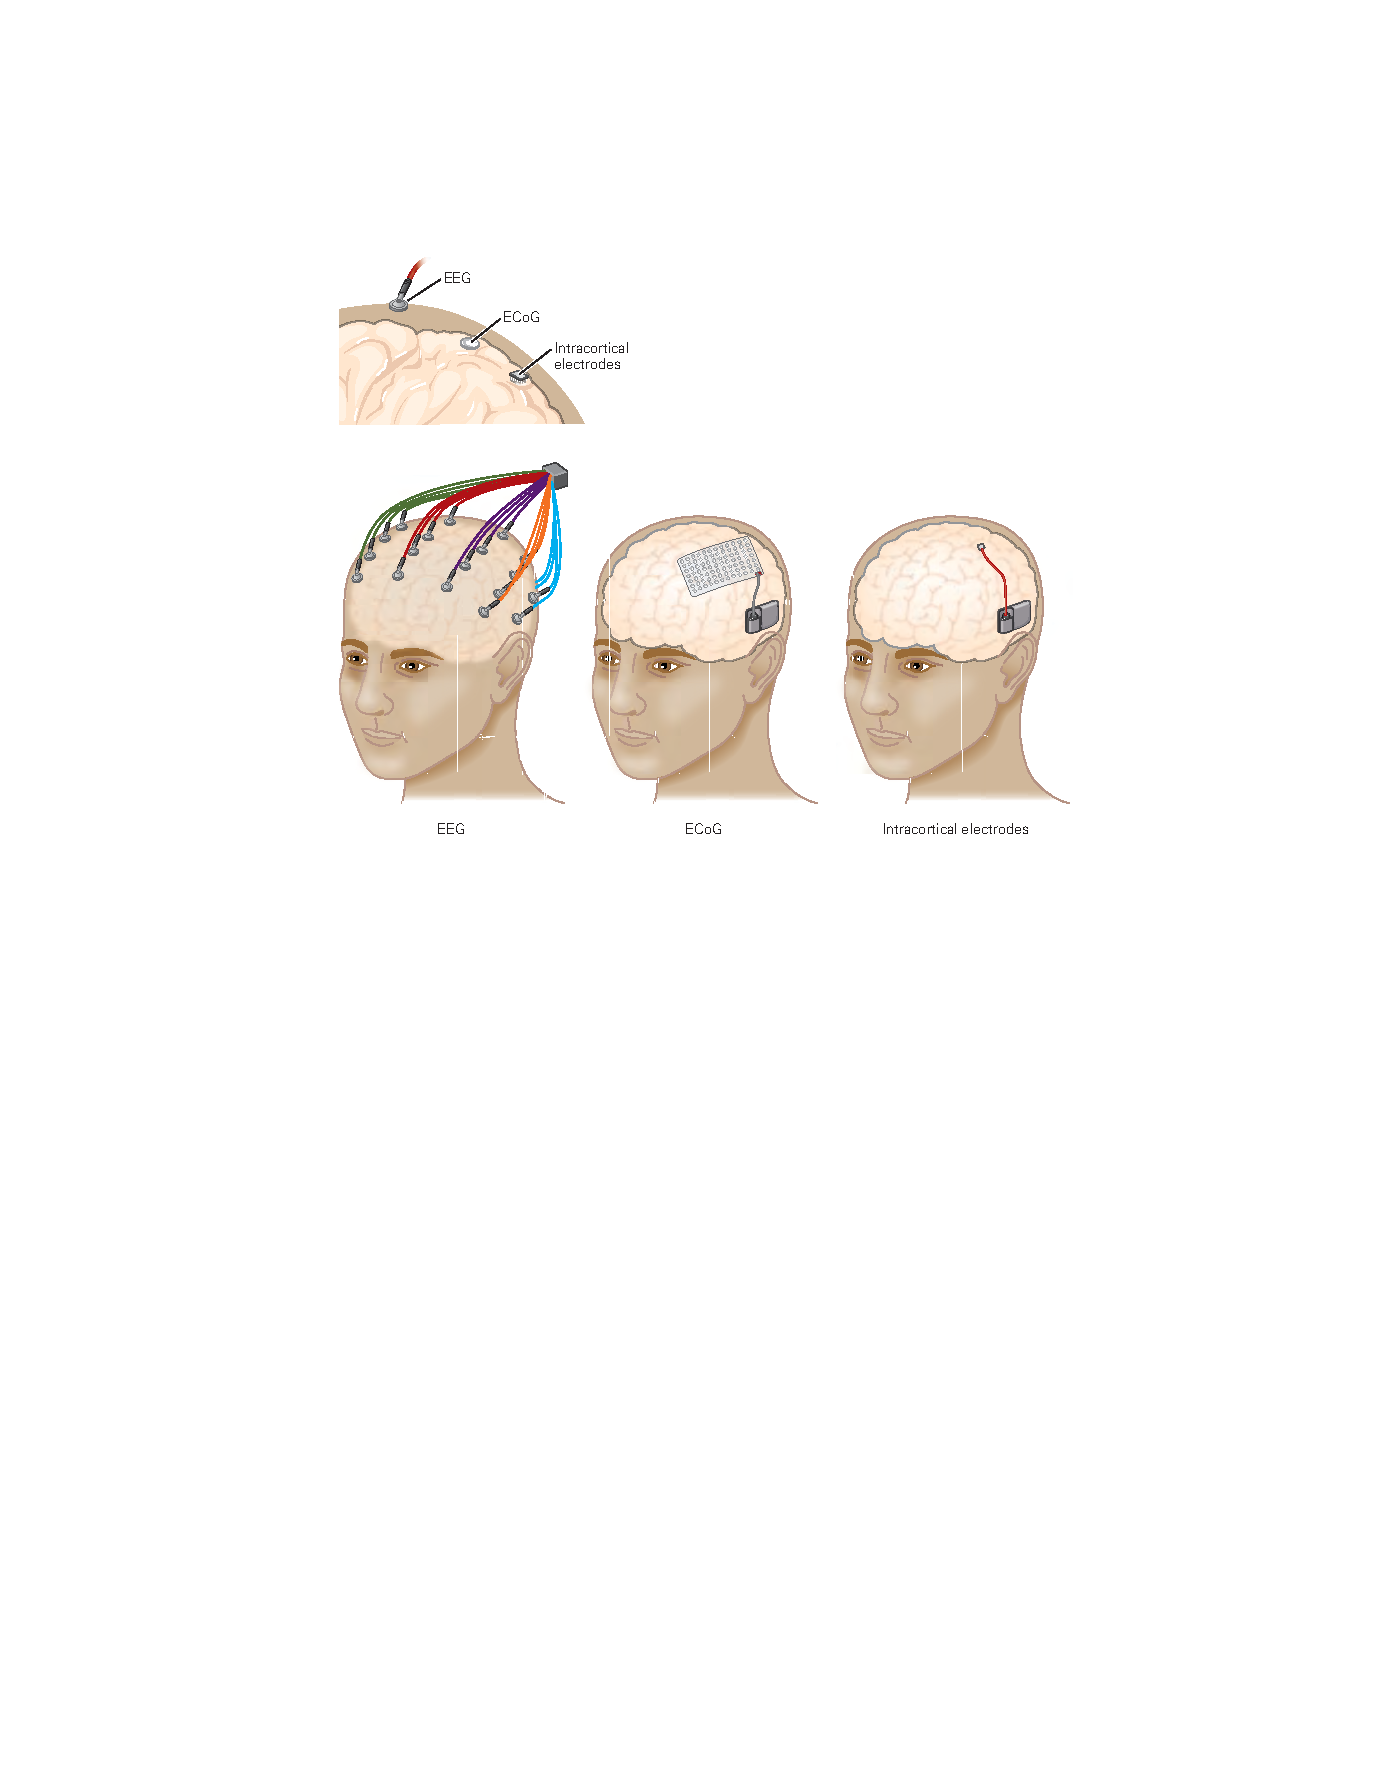
\includegraphics[width=0.5\linewidth]{chap39/fig_39_2}
	\caption{脑机接口使用不同类型的神经传感器。 
		可以使用各种技术测量电神经信号,从皮肤表面的脑电图 (EEG) 电极到大脑表面的皮层电图 (ECoG) 电极,再到植入皮质外 1 至 2 毫米的皮层内电极。 
		可以测量的信号范围从许多神经元的平均值到较少神经元的平均值,最后到单个神经元的动作电位。 (经许可改编自 Blabe 等人,2015 年。)}
	\label{fig:39_2}
\end{figure}


最近,已使用植入式电极阵列技术,例如硬膜下皮层电图 (ECoG) 和精细间隔的微型 ECoG 电极。
由于 ECoG 电极位于大脑表面,因此比 EEG 电极更接近神经元,因此 ECoG 具有更高的空间和时间分辨率,从而提供更多信息来控制脑机接口。


最近,我们在本章重点介绍了穿透性皮层内电极阵列。
皮层内电极阵列由硅或其他材料制成,并涂有生物相容性材料。
这些阵列被植入大脑表面,电极尖端深入大脑皮层 1 至 2 毫米。
它们能够记录单个神经元的动作电位,以及每个电极尖端附近的小神经元簇的局部场电位。
电极能够记录高保真信号,因为它们被插入大脑,使电极尖端在神经元的微米范围内。
这有利于脑机接口性能,因为单个神经元是神经系统中的基本信息编码单元,而动作电位是将信息从神经元的输入区域传输到输出区域的数字代码的基本单元。
此外,皮层内电极可以传递电微刺激来破坏神经活动(例如,DBS)或写入替代信息(例如,本体感受或体感信息)。


神经技术的第二个领域是扩大同时测量的神经元数量。 
虽然一个神经元包含一些关于一个人的预期运动的信息,但需要数十到数百个神经元才能更自然地移动脑机接口,甚至需要更多的神经元才能达到运动功能的自然水平。
尽管可以在大脑的许多区域放置电极阵列,从而从多个区域获得更多信息,但一个关键的挑战是测量每个大脑区域内数千个神经元的活动。
为实现这一目标正在进行许多努力,包括使用具有许多微小轴的电极阵列,每个轴沿其长度有数百个电极触点; 许多微小的电极没有物理连接在一起,而是作为独立的岛插入大脑,在头部外传输数据并无线接收能量;
光学成像技术可以通过检测每个神经元的荧光随时间的变化来捕捉数百个或更多神经元的活动。


第三个领域是用于信号采集、无线数据通信和无线供电的低功耗电子设备。
与上述脑机接口系统不同,后者植入了一个被动电极阵列,其中每个电极通过穿过皮肤的连接器连接到外界,未来的脑机接口将像 DBS 系统一样完全植入。
需要电子回路来放大神经信号、将它们数字化、处理它们(例如,检测何时发生动作电位或估计局部场电位功率),并将此信息传输到附近的假肢接收器中。
出于两个原因,必须将功耗降至最低。
首先,消耗的电量越多,电池或无线充电系统需要提供的电量就越多。
因此,电池需要更大、更频繁地更换,无线供电具有挑战性。
其次,使用电力会产生热量,大脑只能忍受轻微的温度升高,才会产生有害影响。
这些权衡类似于智能手机的权衡,智能手机代表了当前可用于低功耗电子产品的最佳技术。


最后一个领域是所谓的监管系统。
在电子硬件上运行的软件是脑机接口的核心。 
一些软件实现了神经解码的数学运算,而其他软件必须倾向于脑机接口整体操作的各个方面。
例如,监控软件应监控一个人是否希望使用假肢(例如,该人是否在睡觉);
如果神经信号发生变化,从而需要重新校准解码器;
以及整体脑机接口性能和安全性。


在讨论了不同脑机接口和正在开发的神经技术的范围之后,在本章的其余部分,我们将重点关注运动和交流脑机接口。 
我们首先描述不同类型的解码算法及其工作原理。
然后,我们描述了脑机接口开发在帮助瘫痪者和截肢者方面的最新进展。 
接下来,我们将考虑感官反馈如何提高脑机接口表现,以及脑机接口如何用作实验范式来解决有关大脑功能的基本科学问题。
最后,我们以关于脑机接口可能出现的伦理问题的警示作为结尾。



\section{脑机接口利用许多神经元的活动来解码运动}

运动的各个方面——包括位置、速度、加速度和力——都编码在整个运动系统的神经元活动中(第~\ref{chap:chap34}~章)。
尽管我们对运动系统中运动编码的理解不完整,但运动的各个方面与神经活动之间通常存在可靠的关系。
这种可靠的关系使我们能够根据神经活动(脑机接口的关键组成部分)来估计所需的运动。


为了研究运动编码,人们通常会考虑单个神经元在针对同一目标的重复运动(称为“试验”)中的活动。
神经元的活动可以在许多试验中取平均值,为每个目标创建尖峰直方图(图~\ref{fig:39_3}A)。
通过比较不同目标的尖峰直方图,可以描述神经元活动如何随产生的运动而变化。
还可以使用尖峰直方图评估神经元是更多地参与运动准备还是运动执行。


\begin{figure}[htbp]
	\centering
	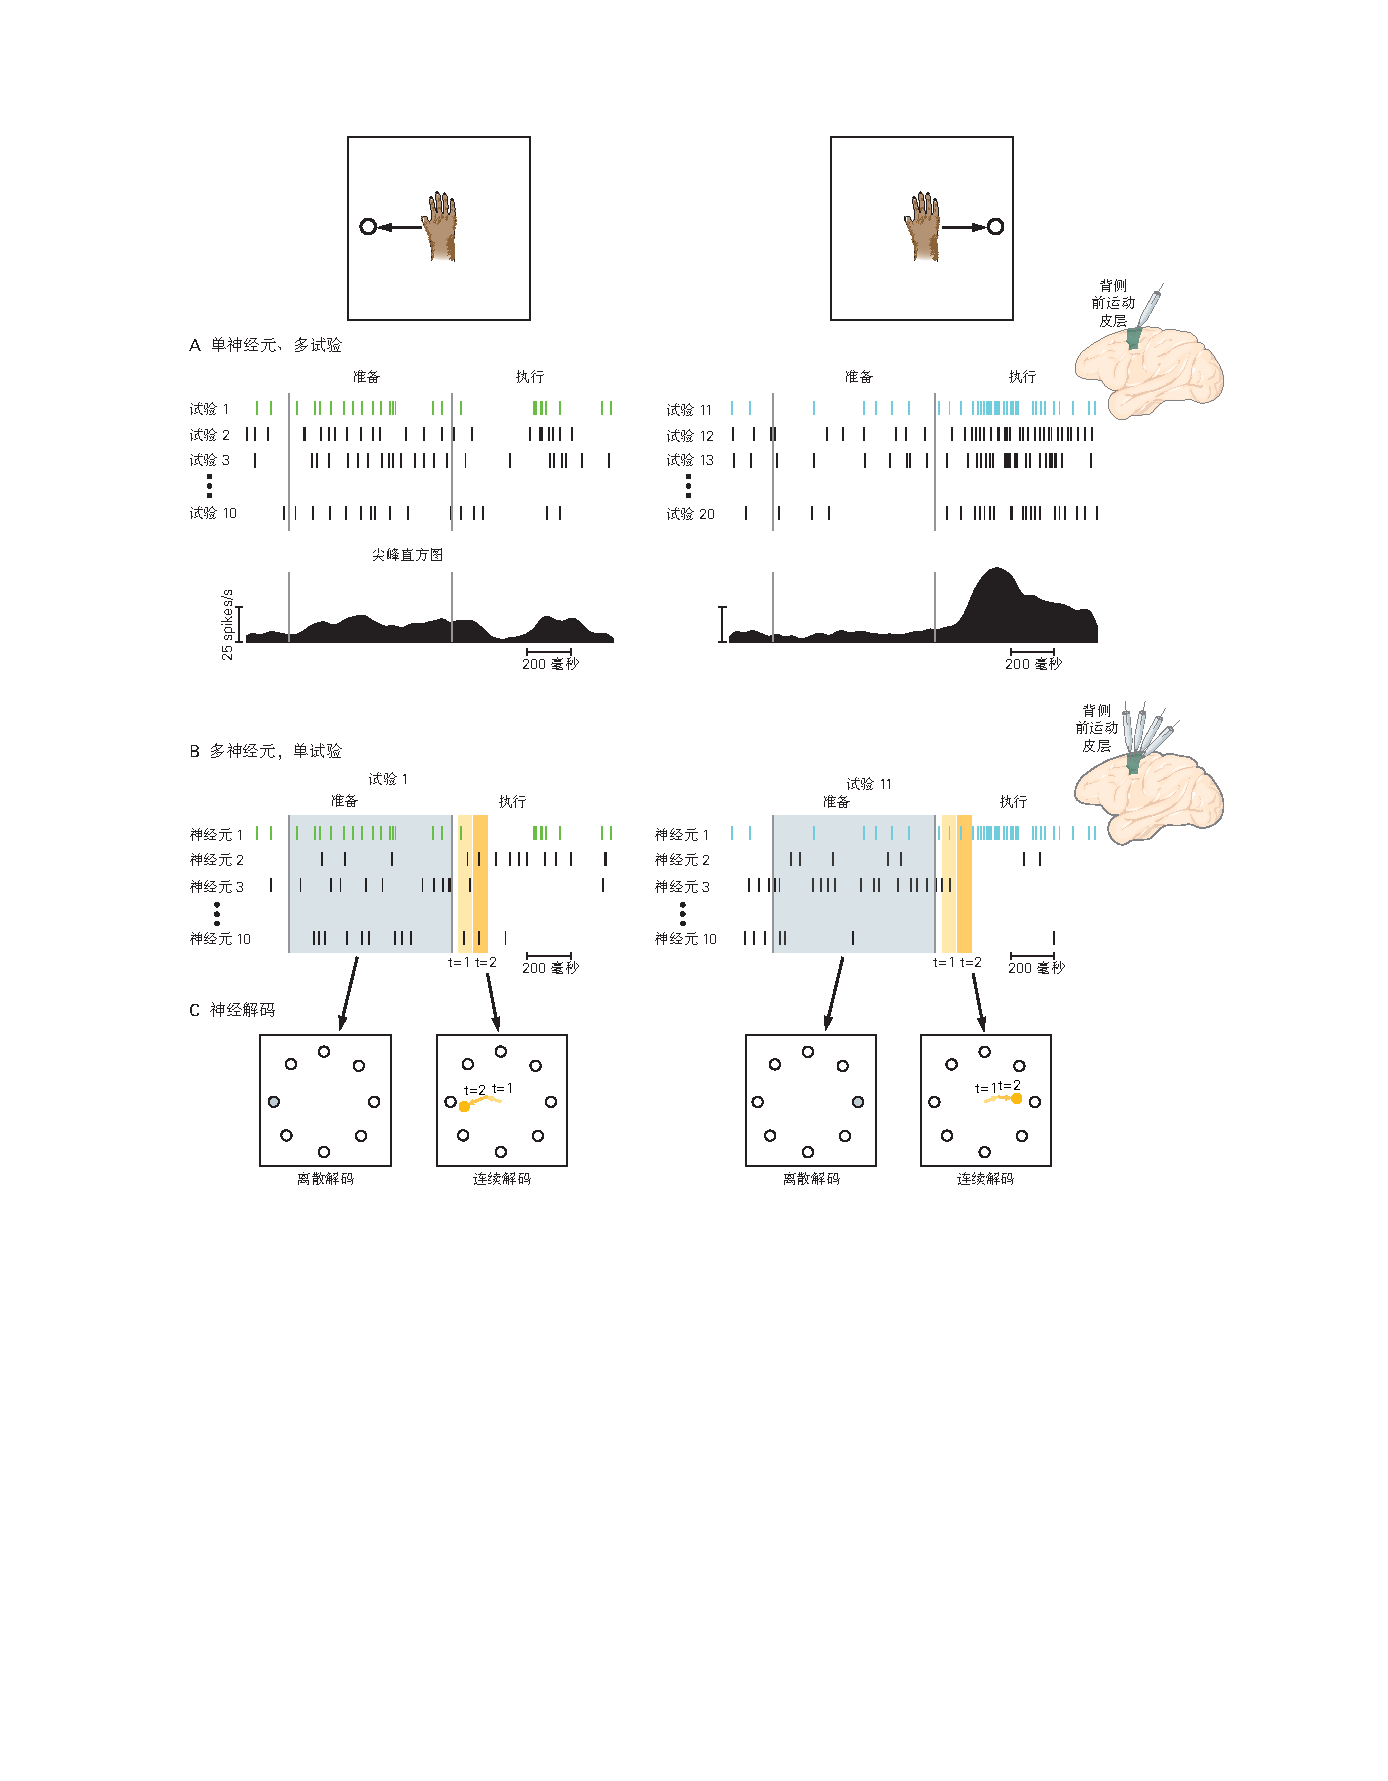
\includegraphics[width=0.5\linewidth]{chap39/fig_39_3}
	\caption{运动编码使用在实验试验中平均的单个神经元的活动,而运动解码使用单个实验试验中许多神经元的活动。
		A. 准备和执行左臂运动(左)和右臂运动(右)的猴子背侧前运动皮层中记录的一个神经元的活动。
		表征神经元的运动编码涉及确定神经元在重复向左或向右运动(每行脉冲序列)中的活动如何与手臂运动的各个方面相关。
		下面是这个神经元向左和向右运动的尖峰直方图,通过对试验中的神经活动进行平均获得。
		该神经元显示出更高水平的向左运动准备活动和更高水平的向右运动执行活动。
		背侧前运动皮层和初级运动皮层中的许多神经元在准备和执行时期都显示出与运动相关的活动,就像所示的神经元一样。
		B. 背侧运动前皮层记录的许多神经元的神经活动,一次向左运动(左)和一次向右运动(右)。
		神经元 1 的尖峰序列对应于 A 部分中所示的尖峰序列。
		尖峰计数是在准备时期进行的,通常在 100 毫秒或更长的大时间段内进行,以估计运动目标。
		相比之下,尖峰计数是在执行时期通常在许多较小的时间段中进行的,每个时间段持续数十毫秒。
		使用如此短的时间段提供了估计运动的每时每刻细节所需的时间分辨率。
		C. 神经解码涉及在单个实验试验中从许多神经元中提取运动信息。 在受试者的工作空间中,有八个可能的目标(圆圈)。
		离散解码(见图 39-5)提取目标位置; 估计目标用灰色填充。
		相反,连续解码(参见图 39-6)提取运动的每时每刻的细节; 橙色点代表某一时刻的估计位置。}
	\label{fig:39_3}
\end{figure}



相比之下,需要在记录神经活动的同时对个体试验执行从神经活动(称为运动解码)估计受试者的期望运动。
单个神经元的活动不能明确提供此类信息。
因此,脑机接口必须在一次试验中监测许多神经元的活动(图~\ref{fig:39_3}B),而不是在多次试验中监测一个神经元的活动。
可以从与运动的准备或执行相关的神经活动中解码所需的运动。
而准备活动与运动目标相关,执行活动则与运动的每时每刻细节相关(第~\ref{chap:chap34}~章)。


跨越多个大脑区域的数百万个神经元协同工作,产生像伸手拿杯子一样简单的动作。
然而,在许多脑机接口中,可以从单个大脑区域记录的数十个神经元的活动中合理准确地解码所需的运动。
尽管这看起来令人惊讶,但事实是运动系统具有大量冗余——许多神经元携带关于所需运动的相似信息(第 ~\ref{chap:chap34}~章)。
这是合理的,因为数百万个神经元参与控制数十块肌肉的收缩。
因此,控制手臂运动的背侧前运动皮层和初级运动皮层区域中的大多数神经元都提供有关大多数手臂运动的信息。


在解码运动时,一个神经元的活动仅提供关于运动的不完整信息,而许多神经元的活动可以提供关于运动的更准确的信息。
这适用于与运动准备和执行相关的活动。
使用多个神经元有助于解码的原因有两个。
首先,一个典型的神经元本身不能明确地确定预期的运动方向。
考虑一个神经元,其活动(在准备或执行期间)通过余弦函数与运动方向相关,称为调谐曲线(图~\ref{fig:39_4}A)。
如果这个神经元以每秒 30 个脉冲的速度发射,则预期的运动方向可能是 120° 或 240°。
然而,通过从调谐曲线不同于第一个神经元的第二个神经元进行记录,可以更准确地确定运动方向。
如果第二个神经元每秒发射 5 个尖峰,对应于 60° 或 120° 方向的运动,则两个神经元之间唯一一致的运动方向是 120°(图~\ref{fig:39_4}B)。
因此,通过同时记录这两个神经元,可以比从一个神经元记录更准确地确定预期的到达方向。
(但是,由于噪声的原因,两个神经元不一定提供对预期到达方向的完美估计,如下所述。)


\begin{figure}[htbp]
	\centering
	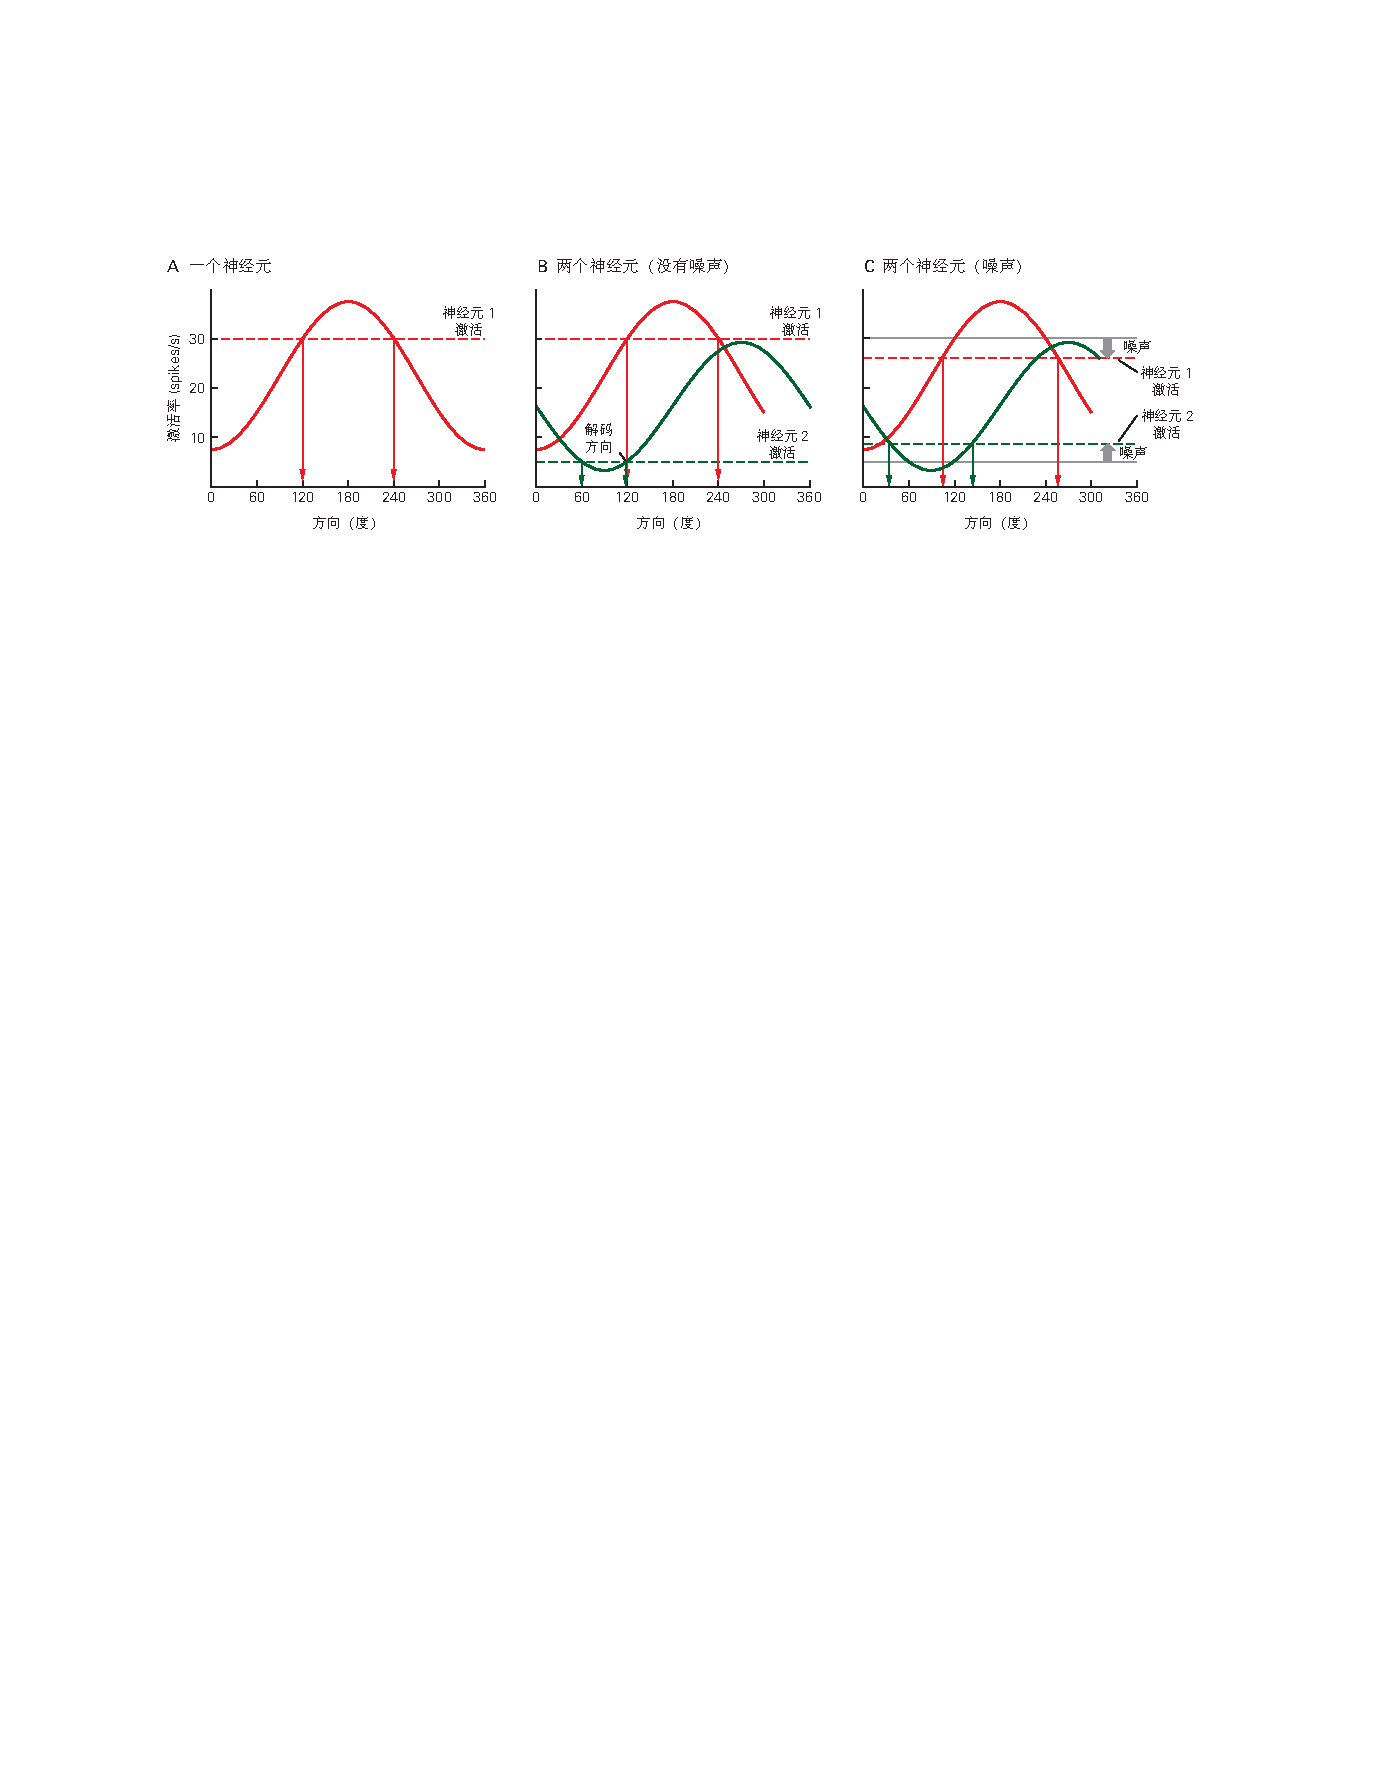
\includegraphics[width=0.5\linewidth]{chap39/fig_39_4}
	\caption{准确的运动解码需要不止一个神经元。
		A. 一个神经元的调谐曲线定义了神经元的活动如何随运动方向变化。
		如果此神经元显示 30 个尖峰/秒的活动,则它可能对应于 120° 或 240° 方向的运动。 
		B. 具有不同调谐曲线的第二个神经元(绿色)显示 5 个尖峰/秒的活动,这可能对应于 60° 或 120° 方向的运动。
		唯一与两个神经元的活动一致的运动方向是 120°,这被确定为解码方向。
		C. 因为神经活动是“嘈杂的”(表示为虚线的垂直位移),通常不可能从两个神经元的活动中最终确定运动方向。
		在这里,没有一个运动方向与两个神经元的活动一致。}
	\label{fig:39_4}
\end{figure}


从多个神经元的活动中解码一个运动可以提供更高准确性的第二个原因是,一个神经元的活动水平通常会随着同一方向的重复运动而变化。
这种可变性通常称为尖峰“噪声”。
假设由于尖峰噪声,第一个神经元以每秒略低于 30 个尖峰的速度发射,而第二个神经元以每秒略高于 5 个尖峰的速度发射(图~\ref{fig:39_4}C)。
在这些条件下,没有一个运动方向与两个神经元的活动水平一致。
相反,必须在两个神经元之间做出妥协,以确定与它们的活动尽可能一致的运动方向。
通过将这个概念扩展到两个以上的神经元,随着神经元数量的增加,可以更准确地解码运动方向。



\subsection{解码算法根据神经活动估计预期运动}

运动解码器是脑机接口的核心组件。 
有两种类型脑机接口的解码器:离散型和连续型(图 39-3C)。
离散解码器估计几个可能的运动目标之一。
这些运动目标中的每一个都可以对应于键盘上的一个字母。
离散解码器解决了统计中的分类问题,可以应用于准备活动或执行活动。
连续解码器估计运动轨迹的每时每刻的细节。
例如,这对于绕过障碍物或转动方向盘很重要。
连续解码器解决了统计学中的回归问题,通常应用于执行活动而不是准备活动,因为可以从执行活动中更准确地估计运动的每时每刻的细节(第~\ref{chap:chap34}~章)。


电机脑机接口必须尽可能准确地生成运动轨迹以实现所需的运动,并且通常使用连续解码器来执行此操作。
相比之下,通信脑机接口关注的是使个人能够尽可能快地传输信息。
因此,选择移动目标(或键盘上的键)的速度和准确性至关重要。
通信脑机接口可以使用离散解码器直接选择键盘上的所需键,或使用连续解码器连续将光标引导至所需键,其中只有最终敲击的键才真正有助于信息传递。
这种看似微妙的区别具有影响所需神经活动类型的含义,因此会影响目标大脑区域,以及所使用的解码器类型。


神经解码涉及两个阶段:校准和持续使用。
在校准阶段,神经活动和运动之间的关系由统计模型表征。
这可以通过在瘫痪者尝试移动、想象移动或被动观察计算机光标或机器人肢体的移动时记录神经活动来实现。
一旦定义了关系,就可以使用统计模型来解码新观察到的神经活动(持续使用阶段)。
持续使用阶段的目标是找到与观察到的神经活动最一致的运动(图~\ref{fig:39_4}B、C)。



\subsection{离散解码器估计运动目标}

我们首先定义一个群体活动空间,其中每个轴代表一个神经元的放电率。
在每次试验(即运动重复)中,我们可以测量特定时期内每个神经元的放电率,它们一起在总体活动空间中产生一个点。
在涉及多个运动目标的许多试验中,人口活动空间中会有分散的点。
如果神经活动与运动目标相关,则点将根据运动目标在种群活动空间中分离(图 39-5A)。
在校准阶段,将人口活动空间划分为不同区域的决策边界由统计模型确定。
每个区域对应一个运动目标。


\begin{figure}[htbp]
	\centering
	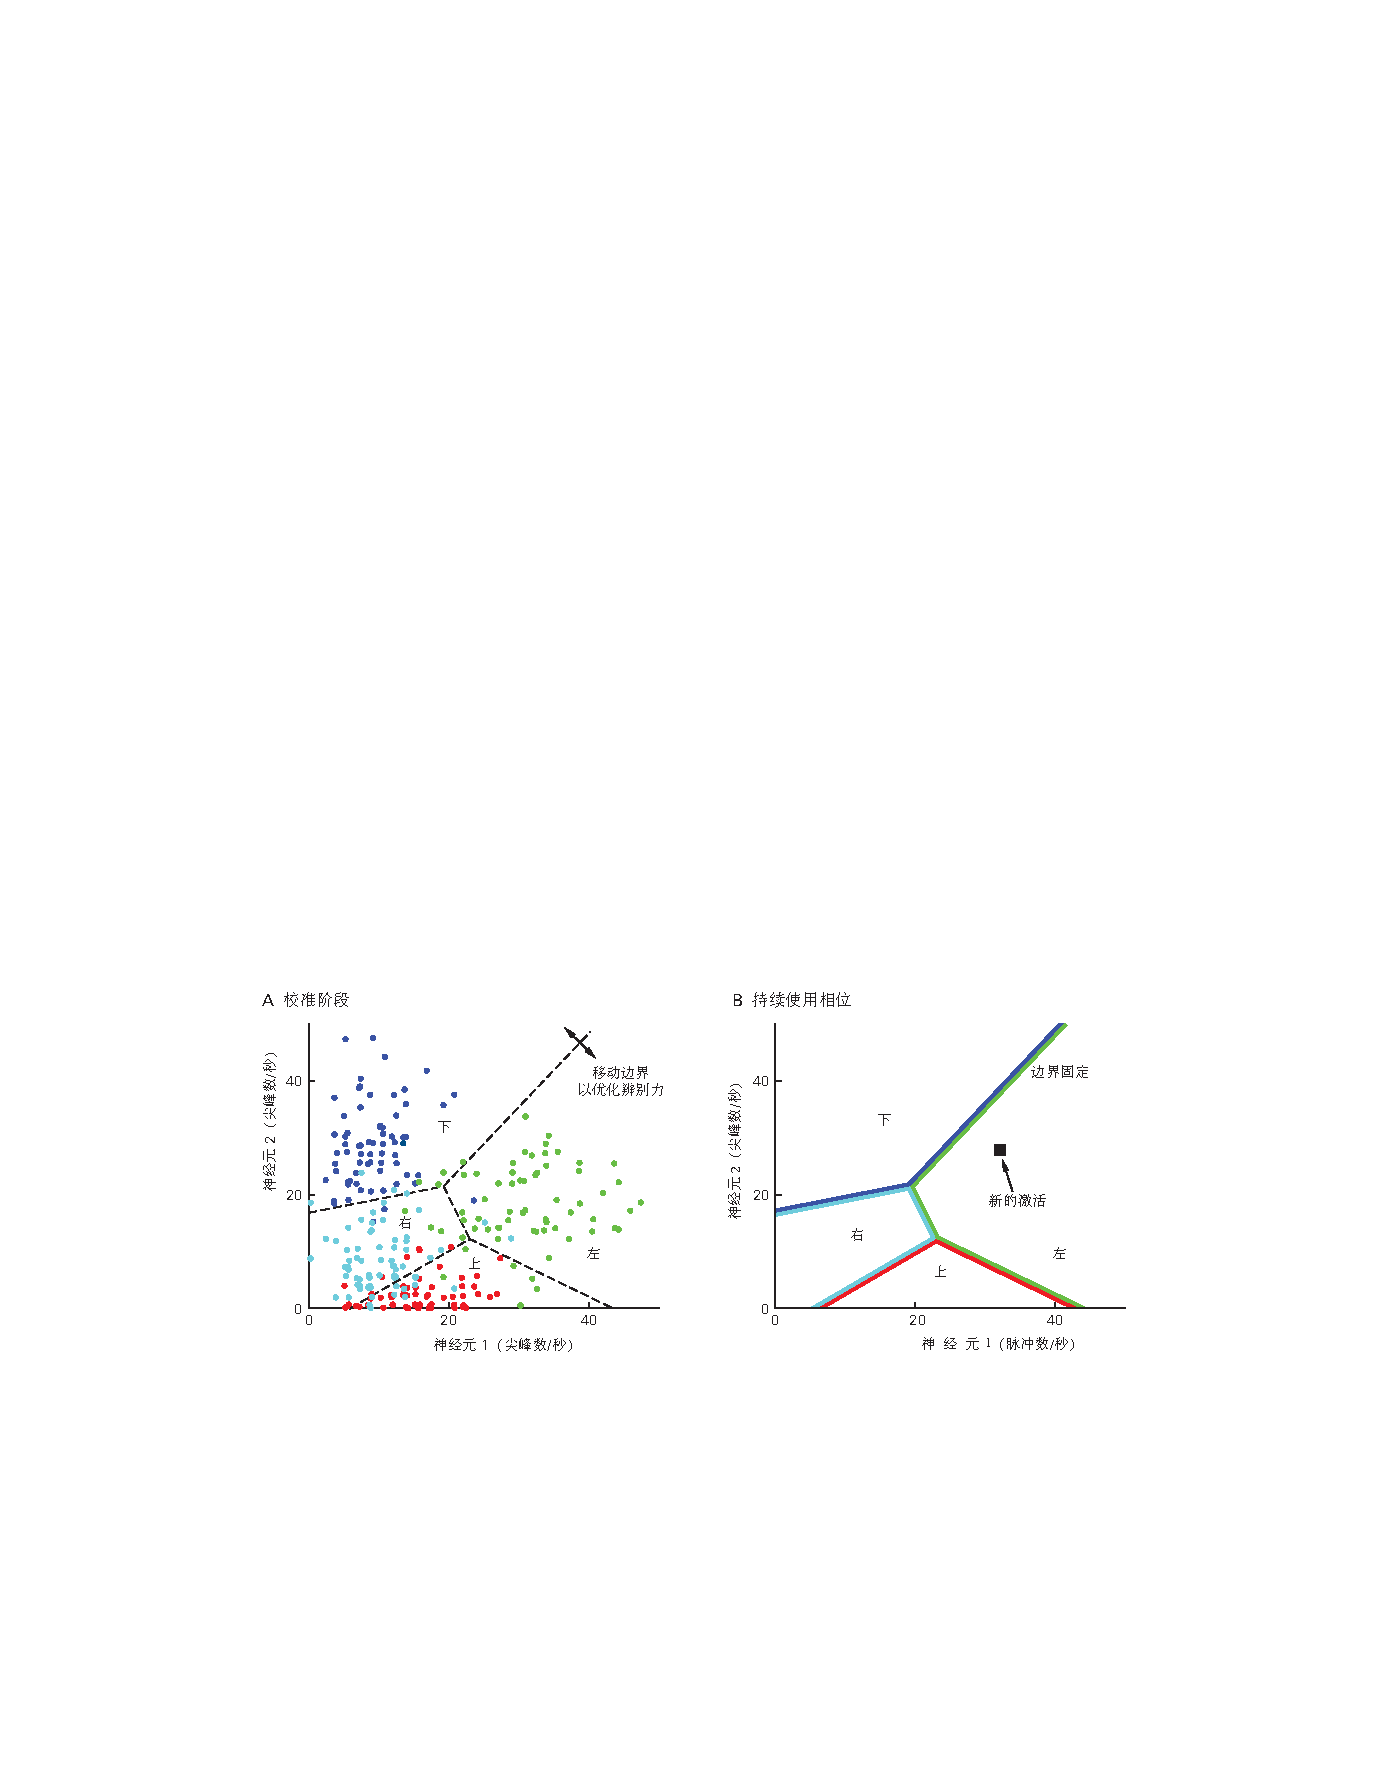
\includegraphics[width=0.5\linewidth]{chap39/fig_39_5}
	\caption{离散解码。
		A. 校准阶段。
		显示了两个神经元的群体活动空间,其中每个轴代表一个神经元的放电率。
		在每次试验(即运动重复)中,两个神经元的活动共同定义了群体活动空间中的一个点。
		每个点都由运动目标着色,这在校准阶段是已知的。 
		决策边界(虚线)由统计模型确定,以优化运动目标之间的区分。
		决策边界为每个移动目标定义了人口活动空间中的一个区域。
		B. 持续使用阶段。
		在此阶段,决策边界是固定的。
		如果我们记录运动目标未知的新神经活动(正方形),则运动目标由神经活动所在的区域决定。
		在这种情况下,神经活动位于与向左目标对应的区域,因此解码器会猜测主体打算移动到向左目标。}
	\label{fig:39_5}
\end{figure}



在持续使用阶段,我们测量运动目标未知的新神经活动(图~\ref{fig:39_5}B)。
解码后的运动目标由神经活动所在的区域决定。
例如,如果神经活动位于对应于向左目标的区域内,则离散解码器会猜测受试者打算在该试验中移动到向左目标。 
即使记录的活动位于与左侧目标相对应的区域内,受试者也可能打算移动到右侧目标。
在这种情况下,离散解码器会错误地估计主体的预期运动目标。
解码精度通常随着同时记录的神经元数量的增加而增加。



\subsection{连续解码器估计运动的每时每刻细节}

手臂位置、速度、加速度、力和手臂运动的其他方面可以使用此处描述的方法以不同的精度级别进行解码。
具体而言,我们将讨论解码运动速度,因为它是运动皮层神经元活动中最强烈反映的量之一,也是大多数脑机接口系统设计的起点。


考虑一群神经元,其活动水平指示运动速度(即速度和方向)。
在校准阶段,为每个神经元确定一个“推动矢量”(图~\ref{fig:39_6}A)。
推动矢量表示神经元的活动如何影响运动速度。 各种连续解码算法的不同之处在于它们如何确定推送向量。
最早的解码算法之一,人口向量算法 (PVA),分配每个神经元的推动向量以指向神经元的首选方向(见图 34-22A)。
神经元的首选方向定义为神经元显示最高活动水平的运动方向(即,图~\ref{fig:39_4} 中的曲线峰值)。
许多关于脑机接口的开创性工作都使用了 PVA。
然而,PVA 没有考虑尖峰噪声的特性(即它在神经元之间的方差和协方差),这会影响解码运动的准确性。
更准确的解码器,即最佳线性估计器 (OLE),结合尖峰噪声的特性来确定推动向量。


\begin{figure}[htbp]
	\centering
	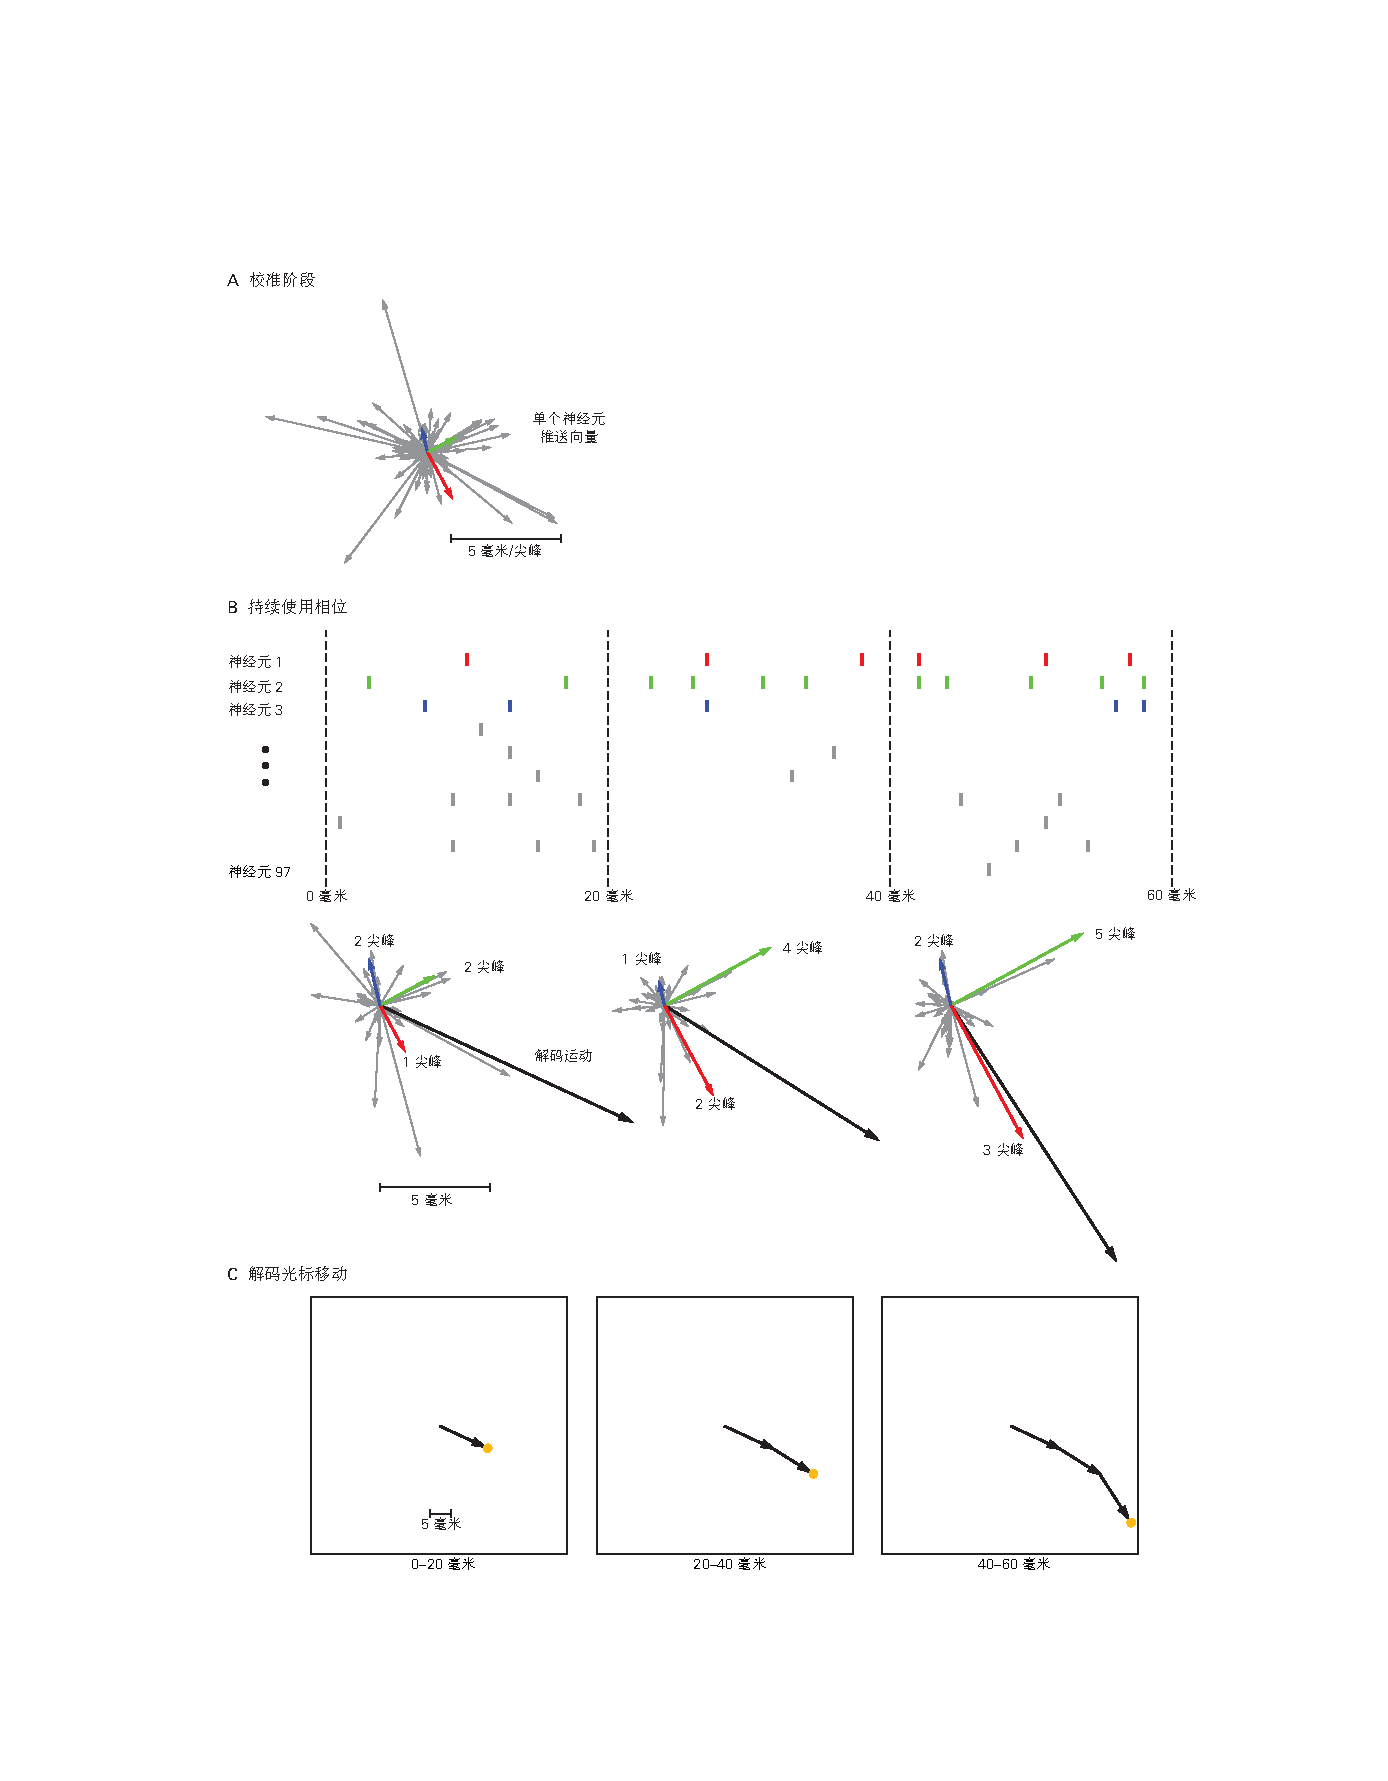
\includegraphics[width=0.5\linewidth]{chap39/fig_39_6}
	\caption{(相反)连续解码。
		A. 在校准阶段,为 97 个神经元中的每一个确定一个推动向量。
		每个向量代表一个神经元并指示来自该神经元的一个脉冲如何驱动每个时间步长的位置变化(即速度)。
		因此,绘图的单位是在一个时间步长内每个尖峰的毫米数。
		不同的神经元可以有不同大小和方向的推动向量。
		B. 在持续使用过程中,在运动执行过程中,尖峰记录来自与面板 A 中相同的神经元。
		在每个时间步长,箭头的新长度是通过从面板 A 中的先前长度开始并按该时间步长中相同颜色的神经元产生的尖峰数缩放来获得的。
		如果一个神经元不发射,则在该时间步内没有指向该神经元的箭头。
		解码后的运动(黑色箭头)是缩放后的推动向量的向量和,表示一个时间步长期间的位置变化(即速度)。
		对于给定的神经元,其缩放推动向量的方向在所有时间步长中都是相同的。
		然而,缩放推动向量的幅度可以从一个时间步长变化到下一个时间步长,具体取决于该神经元的活动水平。
		C. 来自面板 B 的解码运动用于在每个时间步更新计算机光标(橙色点)、机器人肢体或瘫痪肢体的位置。}
	\label{fig:39_6}
\end{figure}


在持续使用阶段,每个推动向量都根据相应神经元在每个时间步长发出的尖峰数进行缩放(图~\ref{fig:39_6}B)。
在每个时间步,解码的运动是所有神经元的缩放推动向量的向量和。
解码后的运动表示一个时间步长期间的位置变化(即速度)。
脑机接口光标(或肢体)位置(图~\ref{fig:39_6}C)然后根据解码的运动进行更新。


为了进一步提高解码精度,每个时间步长的速度估计不仅应考虑当前的神经活动(如图~\ref{fig:39_6}~所示),还应考虑最近的神经活动。
基本原理是运动速度(和其他运动学变量)随时间逐渐变化,因此最近的神经活动应该提供有关运动速度的信息。 
这可以通过在应用 PVA 或 OLE 之前暂时平滑神经活动或使用卡尔曼滤波器来定义描述运动速度(或其他运动学变量)如何随时间平滑变化的统计模型来实现。
使用卡尔曼滤波器,估计速度是当前时间步长的缩放推动矢量(如图~\ref{fig:39_6}B~所示)和前一时间步长的估计速度的组合。
事实上,考虑到最近的神经活动的连续解码算法已被证明比那些不考虑的算法提供更高的解码精度。
卡尔曼滤波器及其扩展广泛用于脑机接口和可用的最准确的连续解码算法。



\section{运动和沟通脑机接口的性能和能力的提高使临床转化成为可能}

瘫痪患者希望进行日常生活活动。
对于无法说话或移动手臂的 ALS 或上脊髓损伤患者,最需要的任务通常是能够进行交流、移动假肢(机器人)手臂或通过刺激肌肉组织来移动瘫痪的手臂。
在描述了如何从大脑的运动区域读出神经信号以及如何解码这些电信号以达到脑机接口控制信号之后,我们现在描述恢复这些能力的最新进展。


大多数实验室研究是在身体健全的非人灵长类动物中进行的,尽管在重要的对照实验中有时会短暂地诱发麻痹。
三种类型的实验范式被广泛使用,在 BMI 校准和持续使用期间指导手臂行为和提供视觉反馈的确切方式不同。
撇开这些差异不谈,我们将在下面重点介绍脑机接口的功能和表现。
我们还重点介绍了最近对瘫痪患者进行的临床试点试验。



\subsection{受试者可以使用通信脑机接口键入消息}

为了研究采用离散解码器和准备活动的通信脑机接口可以多快和准确地运行,猴子被训练来注视和触摸中心目标,并准备到达可能出现在计算机屏幕上几个不同位置之一的外围目标。
使用植入前运动皮层的电极记录尖峰。
在准备时期的特定时间窗口内发生的峰值数量用于预测猴子准备到达的位置(图~\ref{fig:39_7}A)。
如果解码目标与外围目标匹配,则提供液体奖励以表明试验成功。

\begin{figure}[htbp]
	\centering
	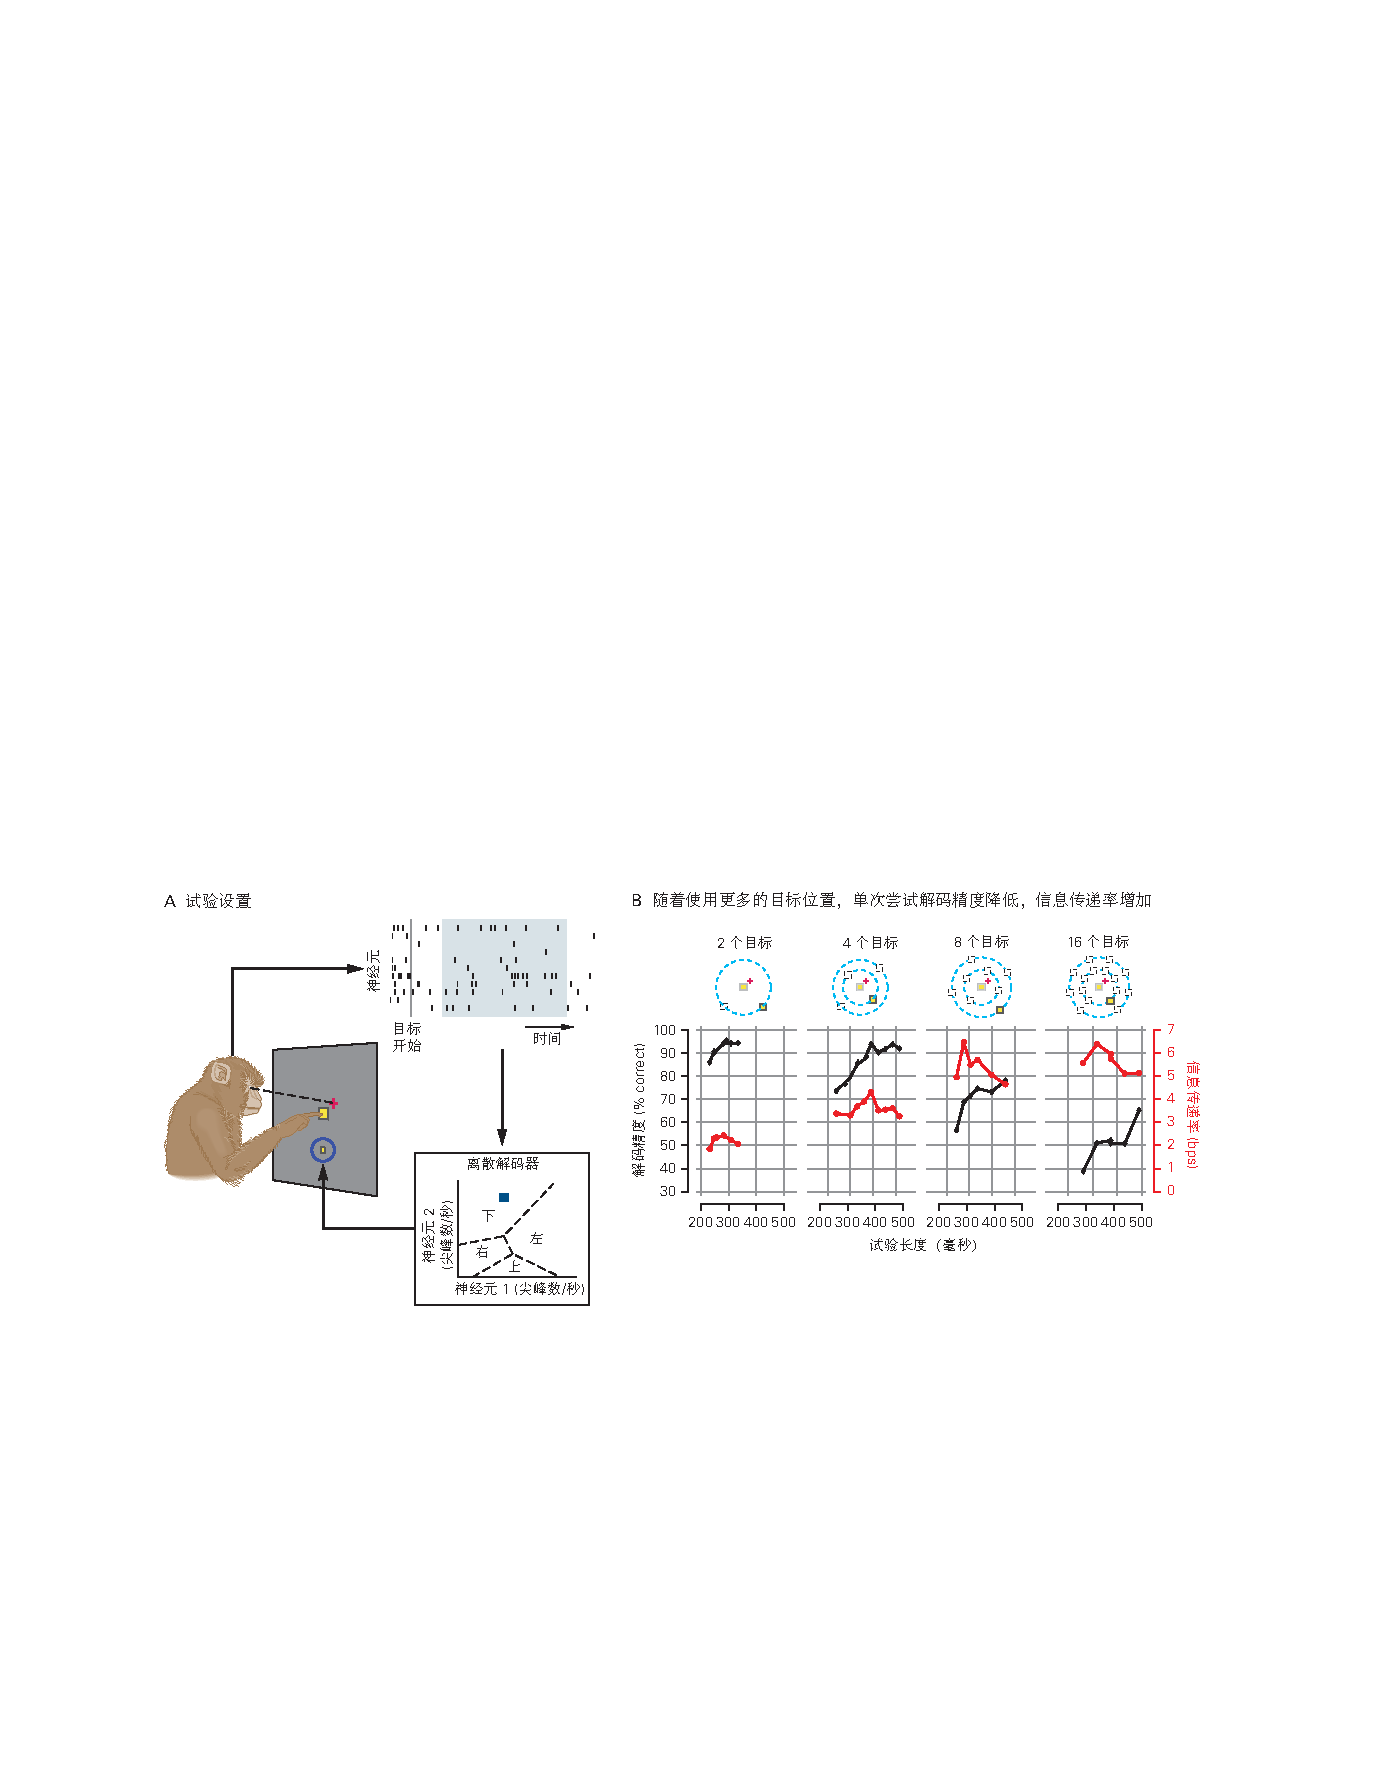
\includegraphics[width=0.5\linewidth]{chap39/fig_39_7}
	\caption{通信脑机接口可以使用基于准备时期神经活动的离散解码器来控制计算机光标。 
		A. 当一只猴子触摸到一个中心目标(黄色大方块)并注视一个中心点(红色+)后,出现了一个外围目标(黄色小方块),猴子准备伸手去拿。 
		尖峰计数是在准备时期进行的,并被输入到一个离散的解码器中。 
		尖峰计数的持续时间(即浅蓝色阴影的宽度)会影响解码性能和信息传输率 (ITR)(参见面板 B)。 
		根据尖峰计数(蓝色方块),离散解码器猜测猴子准备到达的目标。 
		B. 针对不同的试验长度和目标数量显示解码精度(黑色)和信息传输速率(ITR,比特/秒;红色)。 
		试验长度等于尖峰计数的持续时间(在实验期间变化)加上 190 毫秒(在实验期间固定)。 
		后者提供了外围目标的视觉信息到达前运动皮层的时间 (150 ms),加上从神经活动中解码目标位置并在屏幕上呈现解码目标位置的时间 (40 ms)。 (经许可改编自 Santhanam 等人,2006 年。)}
	\label{fig:39_7}
\end{figure}


通过改变尖峰计数的持续时间和可能的目标数量,可以评估目标选择的速度和准确性(图~\ref{chap:39_7}B)。
解码精度往往会随着尖峰计数的周期而增加,因为尖峰噪声在较长的周期内更容易被平均掉。


有效通信的一个重要指标是信息传输率 (ITR),它衡量单位时间内可以传送多少信息。
信息的基本单位是位,由二进制值(0 或 1)指定。
例如,使用三位信息,可以指定 23 = 8 个可能的目标或按键中的哪一个要按下。 
因此,ITR 的度量标准是每秒比特数 (bps)。
ITR 随着尖峰计数的周期增加,然后下降。
原因是 ITR 考虑了选择每个目标的准确度和速度。
除了较长时期的收益递减点之外,准确度的提高速度不足以克服伴随较长时期的目标选择率的下降。


整体性能 (ITR) 会随着可能目标的数量增加而增加,尽管解码精度会降低,因为每个正确的目标选择都会传达更多信息。
这种基于应用于准备活动的离散解码器的设计已经在 BMI 中展示了快速准确的通信。
此 BMI 的 ITR 约为 6.5 bps,相当于每秒大约两到三个目标,准确度超过 90\%。


最近的研究还调查了采用连续解码器和执行活动的通信 BMI 的运行速度和准确度。
评估了两种不同类型的连续解码器:标准卡尔曼滤波器解码运动速度 (V-KF) 和重新校准的反馈意图训练卡尔曼滤波器 (ReFIT-KF)。
V-KF 使用实际手臂运动期间记录的神经活动(即开环控制)进行校准。
ReFIT-KF 通过假设用户希望在每个时间步将光标直接移动到目标,将 BMI 的闭环特性纳入解码器校准。


为了评估性能,两种类型的解码器都用于闭环 BMI 控制(图 39–8A)。
猴子需要将计算机光标从一个中心位置移动到八个外围位置并返回。
通过让猴子也使用手臂运动执行相同的任务,建立了性能评估的黄金标准。
ReFIT-KF 在几个方面优于 V-KF:使用 ReFIT-KF 的光标移动更直,从直线到目标的移动更少; 光标移动速度更快,接近手臂移动的速度(图 39-8B); 并且有更少的(可能令人沮丧的)长期试验。


鉴于其性能优势,ReFIT-KF 正用于瘫痪患者的临床试验(图 39-8C)。
使用植入左侧运动皮层手部控制区的 96 通道电极阵列记录尖峰活动。
信号被过滤以提取动作电位和高频局部场电位,这些电位被解码以提供 BMI 控制光标的“点击”控制。
受试者坐在电脑显示器前,被问到:“你是如何鼓励你的儿子练习音乐的?” 通过尝试移动她的右手,计算机光标在屏幕上移动并停在所需的字母上。
通过试图挤压她的左手,光标下方的字母被选中,就像点击鼠标按钮一样。


临床试验中的 BMI 性能是通过测量受试者能够输入的预期字符的数量来评估的(图~\ref{fig:39_8}D)。
受试者能够通过使用删除键删除偶尔的错误来证明他们键入的字母是有意的。
这些临床测试表明,使用 BMI 可以以每分钟很多字的速度打字。


\begin{figure}[htbp]
	\centering
	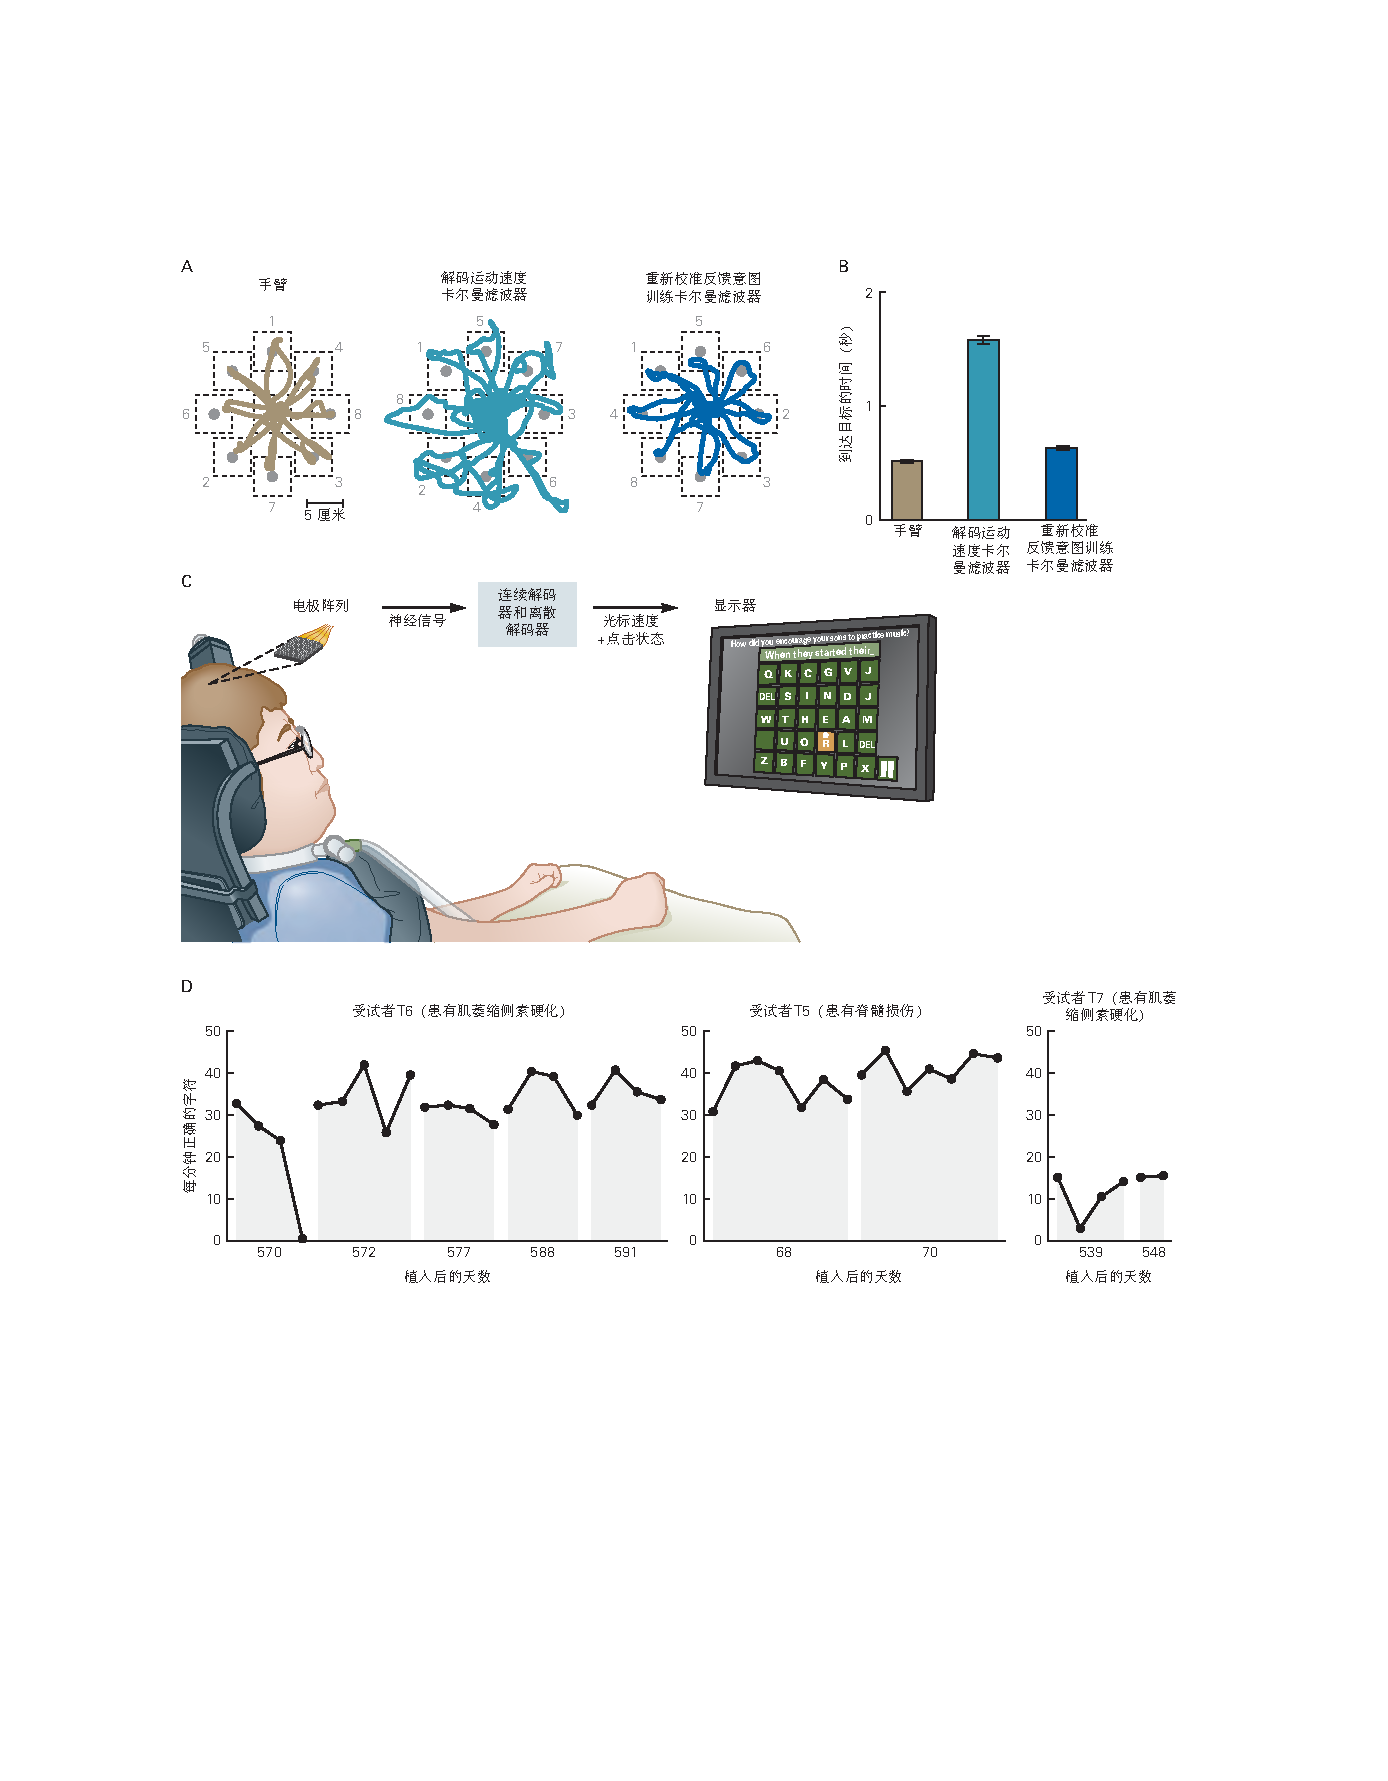
\includegraphics[width=0.5\linewidth]{chap39/fig_39_8}
	\caption{通信脑机接口可以使用基于执行时期神经活动的连续解码器来控制计算机光标。
		A. 比较猴子使用其手臂进行光标控制、估计速度的标准解码器(具有卡尔曼滤波器解码运动速度 [V-KF] 的 BMI)和反馈意图训练的解码器(具有重新校准的反馈意图训练的 Kalman 的 BMI 过滤器 [ReFIT-KF])。
		轨迹显示光标移动到目标和从目标移动,交替显示数字所指示的顺序。在所有河段的持续时间内,痕迹都是连续的。 
		(经 Gilja 等人 2012 年许可改编。)
		B. 在成功试验的中心位置和外围位置之间移动光标所需的时间(平均值 ± 平均值的标准误差)。 
		(经许可改编自 Gilja 等人,2012 年。)
		C. 试点临床试验参与者 T6(53 岁患有肌萎缩性晚期硬化症 [ALS] 的女性)使用 BMI 键入问题的答案。
		(经 Pandarinath 等人许可改编,2017 年。)
		D. 三名临床试验参与者在打字任务中的表现。 性能可以在阵列植入后持续数天甚至数年。 
		(经许可改编自 Pandarinath 等人,2017 年。)}
	\label{fig:39_8}
\end{figure}



\subsection{受试者可以使用脑机接口定向假臂伸手抓取物体}

瘫痪患者喜欢捡起物体,自己进食,并且通常与世界进行身体互动。
带有假肢的运动脑机接口旨在恢复这种失去的运动功能。 
和以前一样,神经活动从大脑解码,但现在被传送到机械臂,手腕在三个维度(x、y 和 z)上移动,手在另一个维度上移动(抓握角度,范围从 张开手到闭合的手)。


在对机械臂的一次测试中,一名瘫痪患者能够利用她的神经活动来引导机械臂伸出手,抓起一瓶液体并将其送至她的嘴中(图~\ref{fig:39_9})。
三维伸展和抓握比自然的手臂和手部动作更慢且更不准确。
重要的是,这表明最初在动物身上开发的相同脑机接口范式,包括测量和解码来自运动皮层的信号,甚至在神经退化或神经损伤发生后数年仍适用于人类。


\begin{figure}[htbp]
	\centering
	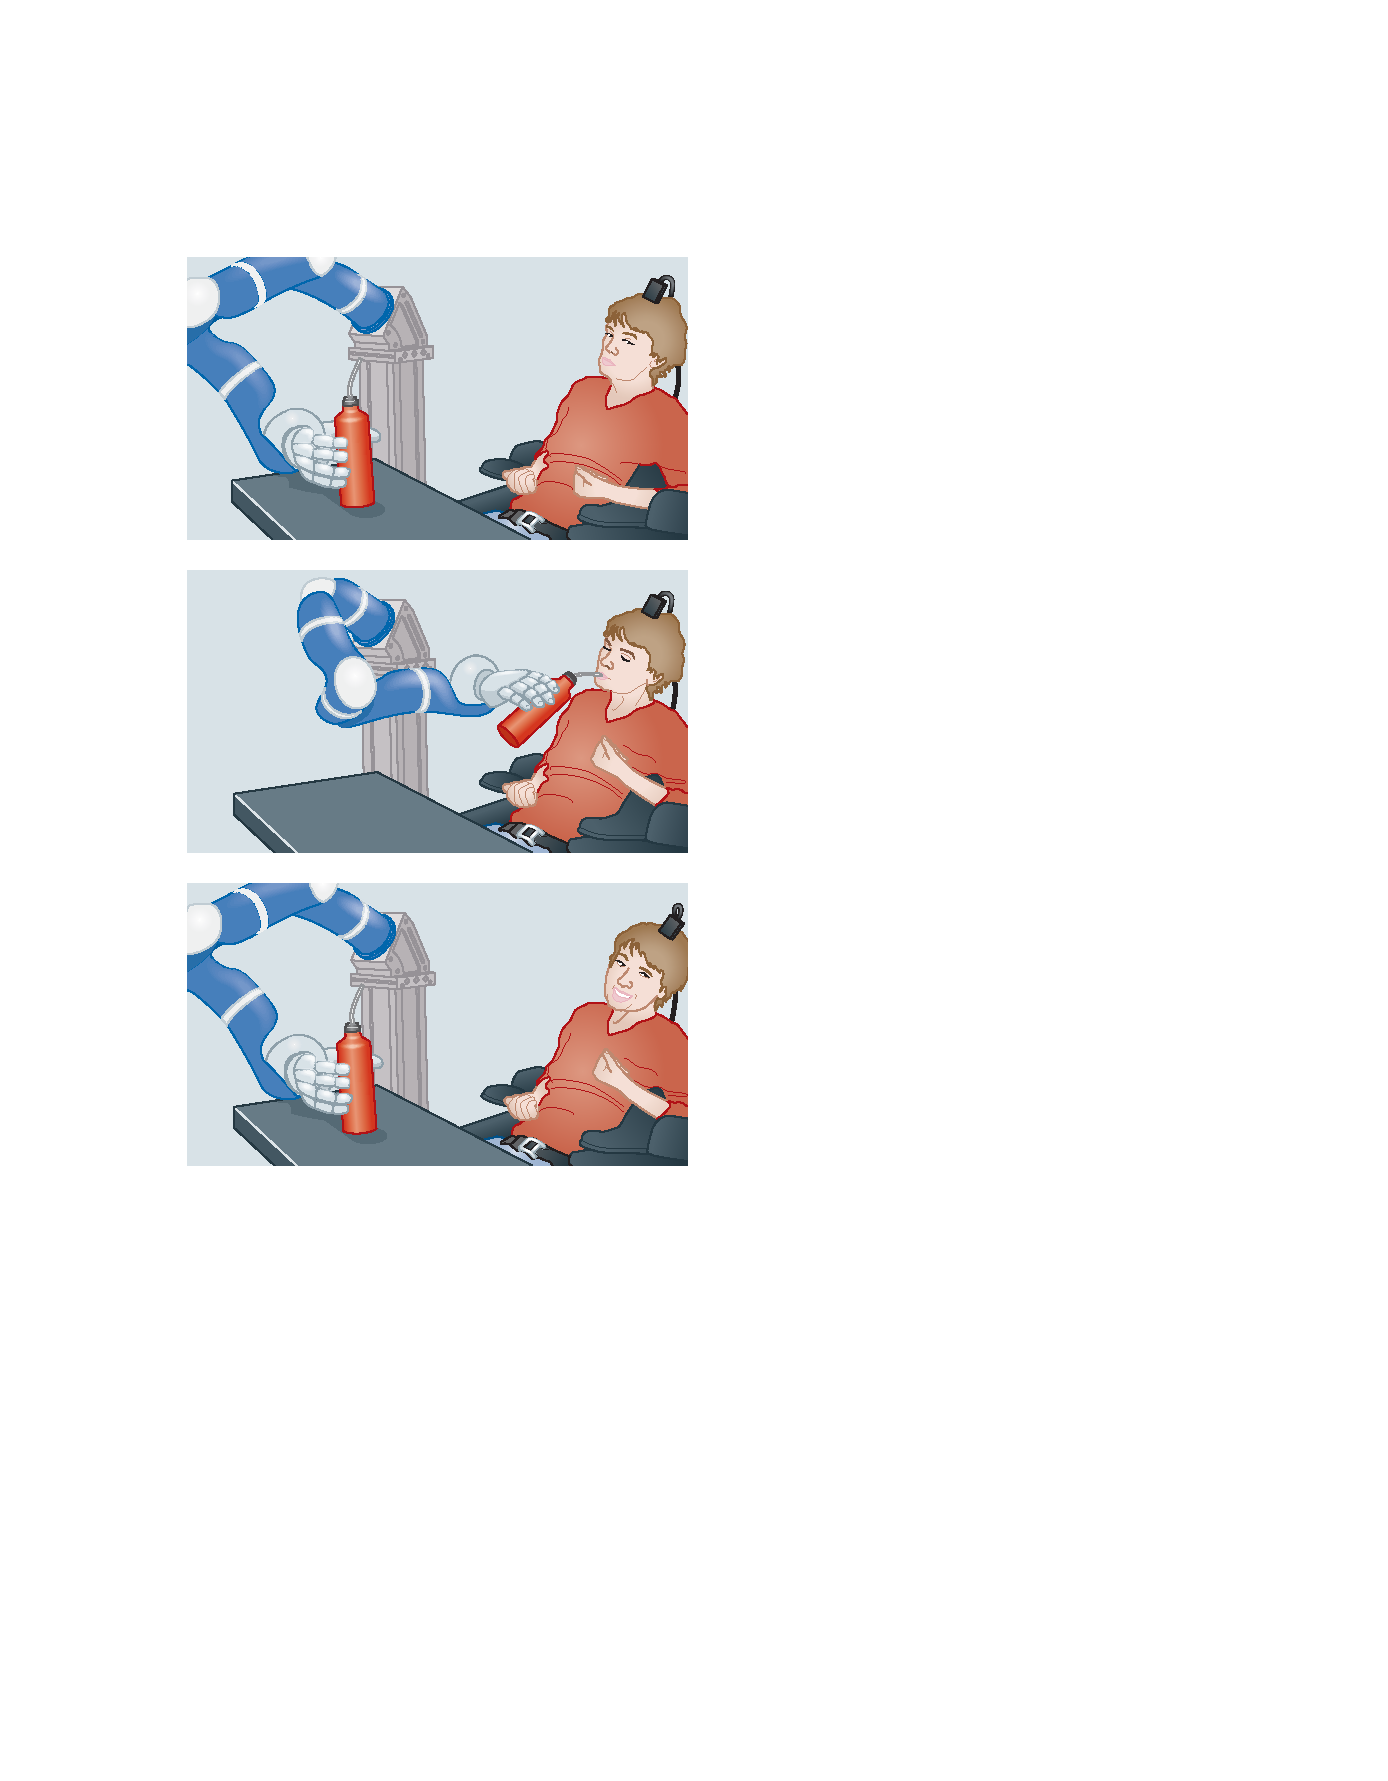
\includegraphics[width=0.5\linewidth]{chap39/fig_39_9}
	\caption{一名瘫痪的受试者使用机械臂从瓶子里喝水,机械臂由使用连续解码器的运动脑机接口控制。 
		第一次成功试验的三张连续图像显示,受试者使用机械臂抓住瓶子,把它放到嘴里,用吸管喝咖啡,然后把瓶子放回桌子上。 
		(改编自 Hochberg 等人,2012 年。)}
	\label{fig:39_9}
\end{figure}


引导假肢和手的脑机接口设备现在能够做的不仅仅是控制三维运动或打开和关闭手。
他们还可以调整手的方向并抓住、操纵和携带物体。
瘫痪者能够以 10 个自由度移动假肢,以抓住不同形状和大小的物体并将它们从一个地方移动到另一个地方(图 ~\ref{fig:39_10})。
抓取和移动物体的完成时间比自然手臂运动要慢得多,但结果令人鼓舞。
这些研究说明了假肢的现有能力以及未来更强大能力的潜力。


\begin{figure}[htbp]
	\centering
	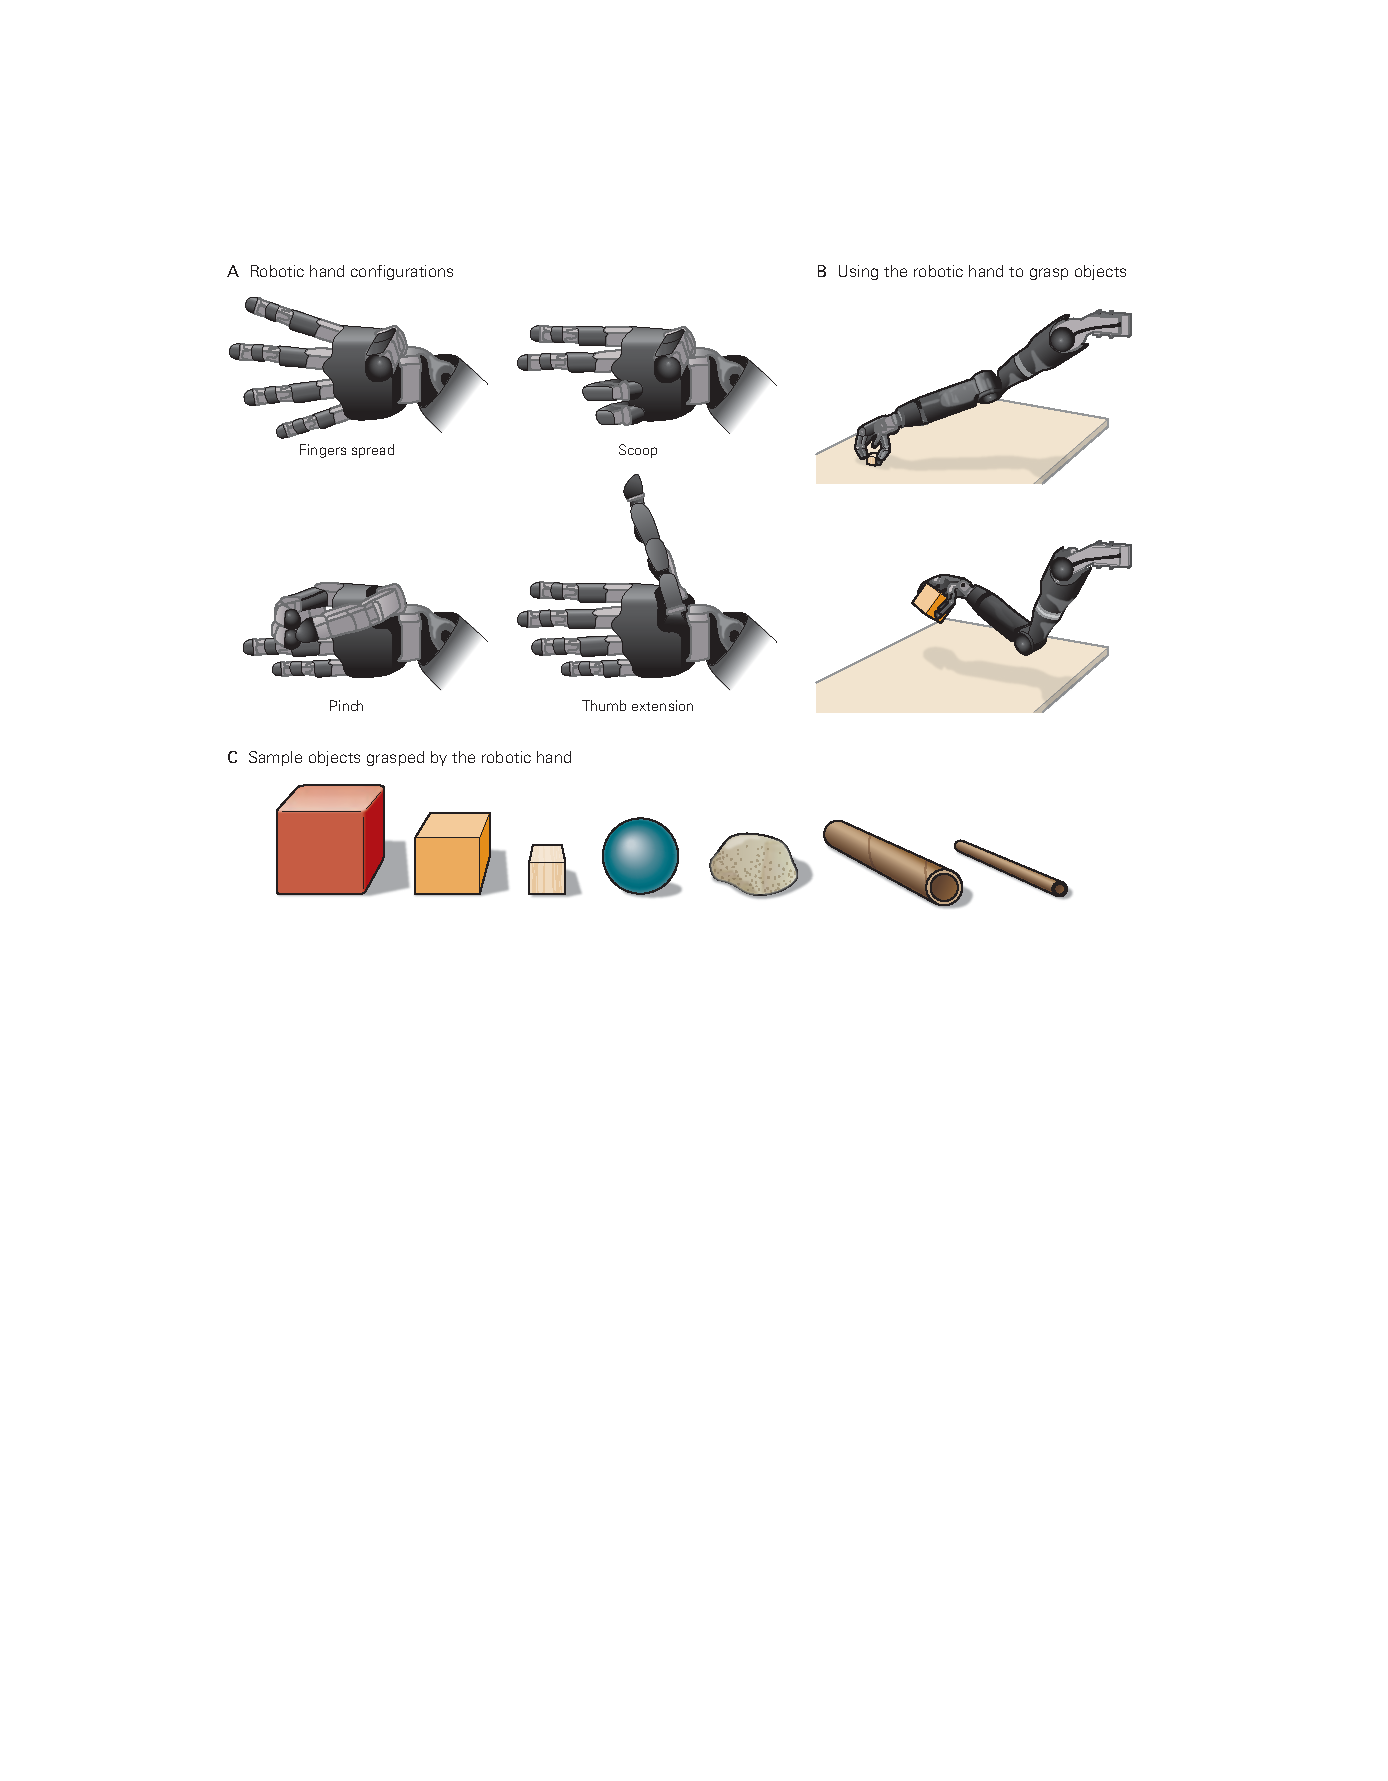
\includegraphics[width=0.5\linewidth]{chap39/fig_39_10}
	\caption{运动脑机接口 (BMI) 可以控制具有 10 个自由度的假肢。 
		A. BMI 指导的不同手部配置示例。
		10 个自由度是三维手臂平移、三维手腕方向和四维手部塑形。
		B. 受试者使用假肢拿起一个物体并移动它。
		C. 使用不同形状和大小的物体来测试BMI的泛化能力。
		(改编自 Wodlinger 等人,2015 年。)}
	\label{fig:39_10}
\end{figure}



\subsection{使用脑机接口定向刺激瘫痪手臂,受试者可以够到并抓住物体}

使用机械臂的另一种方法是恢复生物手臂失去的运动功能。
手臂麻痹是由于脊髓和大脑的神经信号丢失造成的,但肌肉本身通常仍然完好无损,可以通过电刺激使其收缩。
这种能力是功能性电刺激 (FES) 的基础,它通过内部或外部电极向一组肌肉群发送电信号。
通过调整和定时发送到不同肌肉群的电信号,FES 能够以协调的方式移动手臂和手来拾取物体。


对猴子的实验室研究表明,这种基本方法原则上是可行的。
它是通过校准一个连续解码器来预测几块肌肉的预期活动来实现的,这些肌肉会因神经阻滞而暂时瘫痪。
这些预测随后被用于控制相同麻痹肌肉的刺激强度,进而控制运动输出,例如握力角度和力量。
这个过程实际上绕过了脊髓并恢复了对瘫痪的手臂和手的某种自主控制。
最近在使用外部应用或完全植入的最先进的 FES 电极的瘫痪患者身上也得到了类似的结果。
来自运动皮层的皮层内记录信号被解码,以通过 FES 恢复上脊髓损伤患者的运动(图 39-11)。
受试者能够控制不同的手腕和手部运动,包括手指运动,并进行各种日常生活活动。



\section{在脑机接口控制期间,受试者可以使用皮层刺激提供的感觉反馈}

在手臂运动期间,我们依靠多种感官反馈来源来引导手臂沿着所需路径或到达所需目标。
这些来源包括视觉、本体感受和体感反馈。
然而,在大多数当前的脑机接口系统中,用户只能收到有关计算机光标或机器人肢体移动的视觉反馈。
在具有正常运动输出通路但缺乏本体感觉的患者中,手臂运动在运动方向和范围方面远不如健康人准确。
此外,在健康的非人类灵长类动物受试者的脑机接口光标控制测试中,即使不需要手臂运动来移动光标,手臂仍会继续提供本体感受反馈。
当手臂与脑机接口光标一起沿相同路径而不是沿不同路径被动移动时,脑机接口光标控制会更准确。
这证明了“正确的”本体感受反馈的重要性。
基于这两条证据,完全依赖视觉反馈的脑机接口导向运动比正常的手臂运动更慢且更不准确也许就不足为奇了。
这促使最近尝试证明提供替代(即人工)本体感受或体感反馈如何提高脑机接口性能。


一些研究试图通过使用皮层电微刺激来刺激大脑来写入感觉信息。
实验动物可以区分不同频率和振幅的电流脉冲,并且可以利用这种能力通过使用不同的脉冲频率来编码不同的物理位置(类似于本体感觉)或不同的纹理(类似于躯体感觉),从而在脑机接口中提供本体感受或体感信息。
初级体感皮层中的电微刺激可被非人灵长类动物用于在没有视觉的情况下每时每刻地控制光标。
在这些受试者中,与单独使用任何一种感官反馈相比,同时使用电微刺激和视觉反馈导致更准确的运动。


此外,初级体感皮层中的电微刺激也可用于提供触觉信息。
非人灵长类动物在视觉反馈下移动脑机接口定向光标以击中不同的视觉目标,每个目标都会引发不同的刺激频率。 
受试者学会了使用刺激反馈的差异来区分奖励目标和未奖励目标。
这表明电微刺激也可用于在脑机接口控制期间提供体感反馈。


最后,替代体感信息通过电微刺激传递给瘫痪和感觉传入受损的人。
该人报告了他的手和手指的不同位置的自然感觉,这些位置对应于初级体感皮层中不同的刺激位置。



\section{脑机接口可用于推进基础神经科学}

脑机接口正在成为解决有关大脑功能的基本科学问题的越来越重要的实验工具。
例如,人工耳蜗让我们深入了解大脑如何处理声音和言语,语言习得如何影响这些机制的发展,以及神经可塑性如何让大脑解释一些携带贫乏听觉信息的刺激通道。
同样,运动和交流脑机接口有助于阐明感觉运动控制背后的神经机制。
这些科学发现随后可用于改进脑机接口的设计。


脑机接口对基础科学的主要好处是它们可以简化大脑与外界的输入和输出接口,而不会简化人们希望研究的大脑处理的复杂性。
为了说明这一点,考虑控制手臂运动的大脑输出接口。
来自运动皮层和其他大脑区域的数千个神经元将信号沿着脊髓传递到手臂,在那里它们激活肌肉来移动手臂。
了解大脑如何控制手臂运动具有挑战性,因为通常只能记录一小部分向脊髓发送信号的输出神经元,输出神经元的活动与手臂运动之间的关系是未知的,而且手臂有 难以测量的非线性动力学。
此外,通常很难确定哪些记录的神经元是输出神经元。


缓解这一困难的一种方法是使用脑机接口。
由于 BMI 的构建方式,只有那些被记录的神经元才能直接影响光标或机器人肢体的运动。
整个大脑的神经元仍然参与其中,但它们只能通过记录的神经元间接影响光标移动。
因此,与手臂和眼球运动研究相比,人们可以记录脑机接口中的整组输出神经元,并且脑机接口导向的运动可以因果关系归因于所记录神经元活动的特定变化。
此外,记录的神经元活动与光标移动之间的映射由实验者定义,因此是完全已知的。
该映射可以定义为简单的,并且可以在实验期间由实验者轻松更改。
本质上,脑机接口定义了一个简化的感觉运动回路,其组件比手臂或眼球运动更具体地定义和更容易操纵。


脑机接口的这些优势允许研究目前难以使用手臂或眼球运动进行的大脑功能。
例如,一类研究涉及使用脑机接口来研究大脑如何学习。 
脑机接口映射定义了哪些人口活动模式将允许主体成功移动脑机接口定向光标以击中视觉目标。
通过适当定义脑机接口映射,实验者可以挑战受试者的大脑产生新的神经活动模式。


最近的一项研究探讨了大脑更容易和更难产生哪些类型的活动模式。
他们发现,与产生新的活动模式相比,受试者更容易学习现有活动模式和光标移动之间的新关联。
这一发现对我们学习日常技能的能力有影响。
第二类研究涉及询问直接控制运动的神经元活动与不直接控制运动的神经元活动有何不同。
在 BMI 中,可以选择仅使用记录神经元的一个子集(输出神经元)来控制运动。
同时,可以被动监测其他神经元(非输出神经元),而无需用于控制运动。
比较输出和非输出神经元的活动可以深入了解神经元网络如何在内部处理信息并仅将部分信息传递给其他网络。


使用这种范式,最近的一项研究同时记录了初级皮层和纹状体中的神经活动,并将初级运动皮层神经元的一个子集指定为控制 BMI 的输出神经元。
他们发现,在脑机接口学习过程中,与行为最相关的初级运动皮层神经元(输出神经元)优先增加与纹状体的协调,众所周知,纹状体在自然行为中起着重要作用(第~\ref{chap:chap38}~章)。
在使用手臂或眼睛运动的研究中识别输出与非输出神经元将具有挑战性。



\section{脑机接口引发新的神经伦理学考虑}

越来越多的以大脑为中心的生物医学伦理考虑源于我们对神经科学的理解和我们在神经技术方面的能力的急剧扩展。
这些进步是由社会对大脑功能的好奇心推动的,大脑是人体中最不为人所知的器官,以及解决神经系统疾病和损伤患者大量未满足需求的愿望。
脑机接口的使用引发了新的伦理问题,主要有四个原因。


首先,记录高保真信号(即尖峰序列)涉及风险,包括与电极初始植入相关的风险,以及电极和相关植入电子设备在使用寿命期间可能产生的生物(免疫或感染)反应。
长期植入的电极目前的功能寿命约为数月至数年,在此期间,电极周围会形成神经胶质瘢痕组织,电极材料可能会失效。
延长电极功能寿命的努力范围从用新材料制成的纳米级柔性电极到减轻免疫反应,如心脏支架所做的那样。


由于这些原因,考虑接受植入记录技术的患者将需要评估 BMI 的风险和益处,就像所有医疗干预一样。
患者有选择权很重要,因为每个人都有个人偏好,包括愿意接受手术、对功能恢复和结果的渴望以及美容——无论是在考虑癌症治疗还是脑机接口治疗时。
基于不同神经传感器的脑机接口(图~\ref{fig:39_2})具有不同的风险和收益。


其次,由于脑机接口可以以精细的时间分辨率从大脑中读出运动信息,因此它们也有可能读出更多个人和隐私类型的信息。
随着技术变得更加复杂,未来可能出现的神经伦理学问题包括,即使在患者同意的情况下,是否可以读取可能因阿尔茨海默病而丢失的记忆;
通过记录短暂的短期记忆并将它们直接回放到大脑中来促进长期记忆的巩固;
读出潜意识的恐惧或情绪状态,以协助脱敏心理治疗;
或读出可能不会自然发生的预期动作,包括言语。


第三,皮层内写入脑机接口,类似于目前用于减少震颤的 DBS 系统,有一天可能会在大量神经元中唤起自然的时空活动模式。
在极端情况下,一个人可能无法将自我产生的和自愿的神经活动模式与人工或替代模式区分开来。
尽管采用这项技术有许多治疗和有益的原因,例如减少震颤或避免癫痫发作,但可以设想更多可疑的用途,例如征用一个人的运动、感觉、决策或情绪效价回路。


最后,伦理问题还涉及脑机接口运作的限制。
目前的 BMIs 专注于恢复失去的功能,但脑机接口有可能被用来增强超出自然水平的功能。
这就像开了一副比正常视力更好的眼镜,或者开了过量的止痛药,这会导致欣快感,而且往往会让人上瘾。
如果技术上可行,是否应该允许脑机接口使机械臂比自然手臂移动得更快、更准确?
来自脑机接口的连续神经记录,涵盖数小时、数天或数周,是否应该保存以供将来分析,安全和隐私问题与个人基因组数据是否相同或不同?
是否应该购买具有预设内容的脑机接口,例如,在高中时跳过一个数学等级?
身体健全的人是否应该能够选择接受植入式运动脑机接口? 
虽然此类感觉、运动和认知脑机接口治疗的安全和伦理限制似乎显而易见,但社会仍在继续努力解决与其他当前可用医学治疗相关的相同问题。
这些包括增强肌肉组织的类固醇、增强警觉性的能量饮料(例如咖啡因)和改变外观的选择性整形手术。


尽管这些想法和问题中的许多目前可能显得牵强附会,但随着大脑功能和功能障碍的机制不断被揭示,脑机接口系统可以建立在这些发现的基础上,并产生更令人生畏的道德困境。
但同样重要的是,迫切需要通过恢复性脑机接口来帮助患有严重神经系统疾病和损伤的人们。
为了实现正确的平衡,医生、科学家和工程师必须与伦理学家、政府监督机构和患者权益团体进行密切对话和合作。



\section{要点}

1. 脑机接口是读取和/或改变神经元群体水平的电生理活动的医疗设备。
脑机接口可以帮助恢复失去的感觉、运动或大脑处理能力,以及调节病理性神经活动。


2. 脑机接口可以通过刺激神经元向大脑传递感觉信息来帮助恢复失去的感觉能力。
示例包括用于恢复听力的人工耳蜗或用于恢复视力的视网膜假体。


3. 脑机接口可以通过测量许多单个神经元的活动、将此神经信息转换为控制信号以及引导瘫痪的肢体、机器人肢体或计算机光标来帮助恢复失去的运动能力。


4. 电机脑机接口旨在提供对机器人肢体或瘫痪肢体的控制,而通信脑机接口旨在提供与计算机或其他电子设备的快速准确接口。


5. 脑机接口可以通过测量神经活动、处理神经活动并随后刺激神经元来帮助调节病理性神经活动。
示例包括深部脑刺激器和抗癫痫系统。


6. 可以使用不同的技术来测量神经信号,包括脑电图、皮层电图和皮层内电极。
皮层内电极记录电极尖端附近神经元的活动,也可用于传递电刺激。


7. 要研究运动编码,通常要考虑单个神经元在许多实验试验中的活动。
相反,对于运动解码,需要考虑单个实验试验中许多神经元的活动。


8. 离散解码器从神经群体活动中估计几个可能的运动目标之一。
相比之下,连续解码器根据神经群体活动估计运动的每时每刻的细节。


9. 该领域在提高脑机接口的性能方面取得了实质性进展,这是根据估计运动的速度和准确性来衡量的。
现在可以以接近手臂运动的速度和精度的方式移动计算机光标。


10. 除了控制计算机光标外,脑机接口还可以使用功能性电刺激来引导机器人肢体或瘫痪肢体。
对身体健全的非人类灵长类动物进行的临床前实验的发展随后在对瘫痪人群的临床试验中进行了测试。


11. 脑机接口的未来发展将部分取决于神经技术的发展。
这些包括硬件(例如,神经传感器和低功率电子设备)、软件(例如,监控系统)和统计方法(例如,解码算法)方面的进步。


12. 提高脑机接口性能的一个重要方向是为用户提供除视觉反馈之外的其他形式的感官反馈。
当前研究的一个领域是在持续使用期间使用神经元刺激来提供替代感觉反馈,代表体感和本体感觉。


13. 除了帮助瘫痪患者和截肢者外,脑机接口正越来越多地被用作了解大脑功能的工具。
脑机接口简化了大脑的输入和输出接口,并允许实验者定义神经活动和运动之间的因果关系。


14. 脑机接口提出了新的神经伦理学问题,这些问题需要与脑机接口为受伤或疾病患者提供的好处一起考虑。

